\section{Simetría, periodicidad y continuidad del espectro $\Sigma_{x}$}
\label{sec: simetria, periodicidad, continuidad}
Fijada una dimensión $n \geq 2$,
si $x \in \IR^{n}$ es cualquier señal y 
$\Sigma_{x}$
es su espectro como se definió en
\ref{def: espectro monofrecuenciales inicial},
en esta sección vamos a demostrar 
algunos resultados sobre la periodicidad 
de esta función y su simetría 
respecto a puntos de la forma
$\frac{n}{2} \IZ$.
Esto será de utilidad pues nos permitirá
acotar considerablemente el dominio de frecuencias
de $\Sigma_{x}$.



\begin{prop}
\label{prop: periodicidad espectro}
\textbf{(Periodicidad del espectro)}
Sean $n \geq 2$, $x \in \IR^{n}$.
Sea $\Sigma_{x}$ el espectro de $x$ como se definió en 
\eqref{def: espectro monofrecuenciales inicial}.
El espectro $\Sigma_{x}$ es $n-$periódico, es decir, 
para cualquier frecuencia
$0 \leq \omega \leq n$
y toda $K \in \IZ$, se tiene que 
\[
\sigma_{n}(x, \omega) = \sigma_{n}(x, \omega + Kn).
\]
\end{prop}
\noindent
\textbf{Demostración.}
Sólo observe que 
\begin{align*}
\tilde{c}_{n, \omega + Kn} = & \left( cos \left( 2 \pi
\left( \omega + Kn \right) \frac{m}{n} \right) \right)_{m=0}^{n-1} \\
= & \left( cos \left( 
2 \pi \omega \frac{m}{n} + 2 \pi K m
\right) \right)_{m=0}^{n-1} \\
= & \left( cos \left( 
2 \pi \omega \frac{m}{n}
\right) \right)_{m=0}^{n-1} = \tilde{c}_{n, \omega}
\end{align*}
y, similarmente, que 
\[
\tilde{s}_{n, \omega + Kn} = \tilde{s}_{n, \omega},
\]
luego, por definición de los espacios monofrecuenciales
(c.f. ecuación \ref{eq: espacio Pnw}),
\begin{align*}
P_{n, \omega + Kn} =
& span(\tilde{c}_{n, \omega + Kn}, \tilde{s}_{n, \omega + Kn}) \\
= & span(\tilde{c}_{n, \omega }, \tilde{s}_{n, \omega }) = P_{n, \omega};
\end{align*}
de esto se concluye, usando la definición
\ref{def: final de sigmas},
que 
\[
\sigma_{n}(x, \omega) = 
cos (\measuredangle(x, P_{n, \omega}))
= cos (\measuredangle(x, P_{n, \omega + Kn})) = 
\sigma_{n}(x, \omega + Kn).
\]
\QEDB
\vspace{0.2cm}

\begin{figure}[H]
	\sidecaption{
	Según la periodicidad establecida en la proposición 
	\ref{prop: periodicidad espectro}, basta calcular los
	coeficientes espectrales
	$\sigma_{n}(x, \omega)$ para frecuencias
	$0 \leq \omega \leq n$.
	\label{fig: periodicidad espectro}
	}
	\centering
	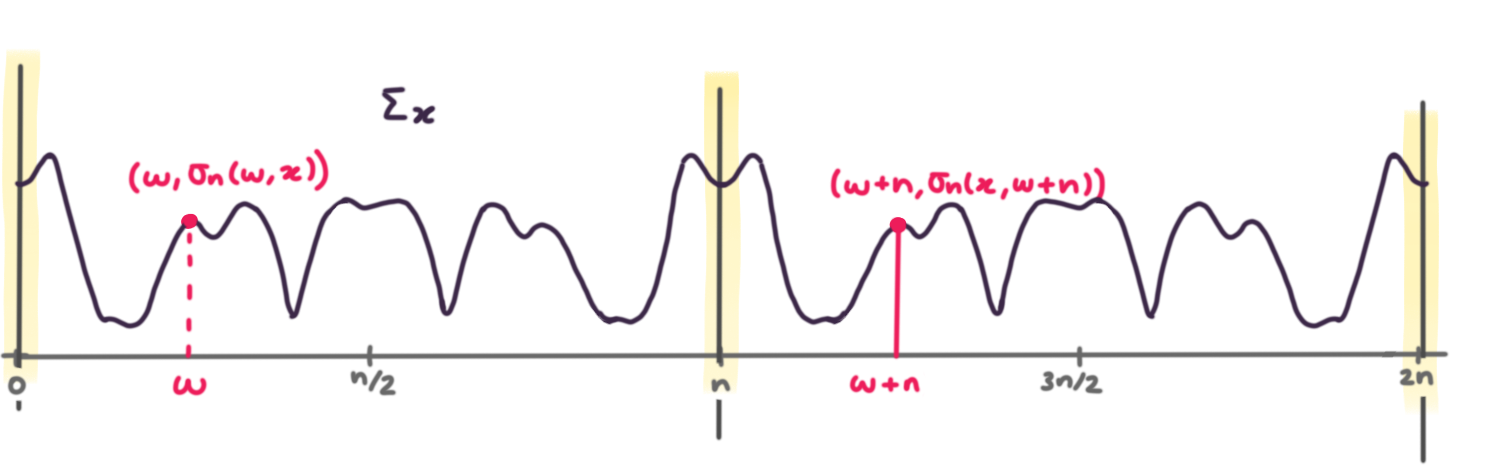
\includegraphics[scale = 0.9]{periodicidad_espectro} 
\end{figure}	


\begin{prop}
\textbf{(Simetría del espectro)}
Sean
$n \geq 2$,
$x \in \IR^{n}$. Para toda $0 \leq1 \omega \leq \frac{n}{2}$,
\[
\sigma_{n}(x, \omega) = 
\sigma_{n}(x, n-\omega ). 
\]
\end{prop}
\noindent
\textbf{Demostración.}
En efecto, 
\begin{align*}
\tilde{c}_{n, \omega + n} = & \left( cos \left( 2 \pi
\left( n- \omega \right) \frac{m}{n} \right) \right)_{m=0}^{n-1} \\
= & \left( cos \left( 
2 \pi n \frac{m}{n} - 2 \pi \omega
\frac{m}{n}
\right) \right)_{m=0}^{n-1} \\
= & \left( cos \left( 
2 \pi m - 2 \pi \omega \frac{m}{n} 
\right) \right)_{m=0}^{n-1} \\
= & \left( cos \left( 2 \pi \omega \frac{m}{n} \right) \right)_{m=0}^{n-1}
= \tilde{c}_{n, \omega}
\end{align*}
y, similarmente,
\[
\tilde{s}_{n, \omega + Kn} = -\tilde{s}_{n, \omega};
\]
de esto, como en la demostración de la proposición
\ref{prop: periodicidad espectro}, se concluye la igualdad
entre los espacios $P_{n, \omega}$ y $P_{n, n-\omega}$, y de esto
la igualdad deseada.
\QEDB
\vspace{0.2cm}

\begin{figure}[H]
	\sidecaption{
	Podemos así afinar la afirmación hecha en la figura 
	\ref{fig: periodicidad espectro} y concluir que basta
	calcular los coeficientes
	$\sigma_{n}(x, \omega)$ para $0 \leq \omega \leq \frac{n}{2}$,
	pues los demás pueden deducirse a partir de reflexiones y traslaciones.
	\label{fig: simetria espectro}
	}
	\centering
	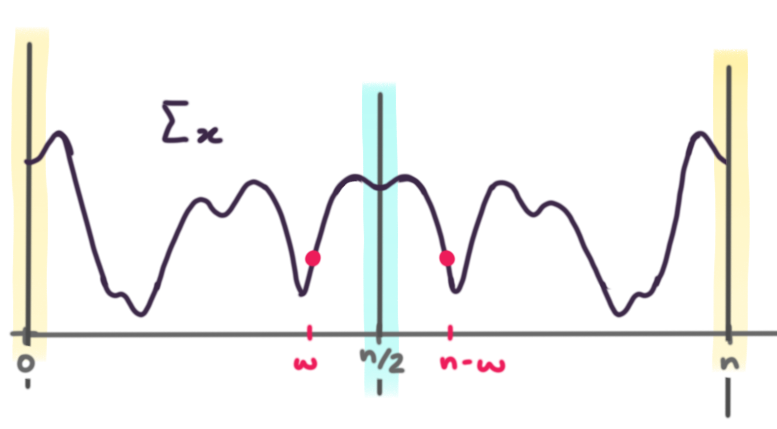
\includegraphics[scale = 1.4]{simetria_espectro} 
\end{figure}	
 

\begin{nota}
\label{nota: muestreo dom frecuencia}
Según estas propiedades de periodicidad y simetría,
podemos limitarnos a evaluar el espectro
$\Sigma_{x}$ de una señal sólo en frecuencias
contenidas en el intervalo $[0, n/2]$, pues los valores
del espectro para otros valores pueden deducirse por periodicidad
y simetría. \\

Ahora bien, para poder escribir programas
para calcular un tal espectro $\Sigma_{x}$
se debe de usar
un conjunto discreto de puntos.
Para los espectros que calcularemos de ahora en 
adelante, adoptamos la convención de 
usar usar como dominio 
del espectro
$\Sigma_{x}$ de una señal $x \in \IR^{n}$
al conjunto
\begin{equation}
\label{eq: malla frecuencias}
\left\{ \frac{a}{100} : \hspace{0.2cm}
0 \leq a \leq 
\left\lfloor\frac{100n}{2}\right\rfloor,
\right\}
\end{equation}

\noindent
es decir, se toman $100$ muestras por
cada unidad del intervalo 
$\left[ 0, \frac{n}{2}\right]$
\end{nota}


Para terminar, hagamos algunos comentarios
sobre la continuidad del espectro $\Sigma_{x}$
de una señal $x \in \IR^{n}$.
Por la periodicidad y simetría del espectro, basta
analizar la continuidad de $\Sigma_{x}$ sólo en el
intervalo cerrado $[0, n/2]$. \\

Será de utilidad introducir la siguiente notación.
\begin{defi}
\label{def: momentos de x}
Sean $n \geq 2$, $x= (x_{m})_{m=0}^{n-1} \in \IR^{n}$, $k \geq 0$.
Se definen a los números $M_{k}(x)$ y 
$\tilde{M}_{k}(x)$ como sigue;
	\begin{equation}
	\label{eq: momento k esimo de x}
	M_{k}(x) := \suma{m=0}{n-1}{m^{k}x_{m}}.
	\end{equation}
	
	\begin{equation}
	\label{eq: momento skew k esimo de x}
	\tilde{M}_{k}(x) := \suma{m=0}{n-1}{(-1)^{m}m^{k}x_{m}}.
	\end{equation}
\end{defi}


\begin{teo}
\label{teo: limite del espectro por cero}
\textbf{(Sobre la continuidad del espectro)}
Sean $n \geq 2$, $x \in \IR^{n}$.
Sea $\Sigma_{x}: [0, n/2] \rightarrow [0,1]$ el espectro de $x$ como se definió
en \ref{def: espectro monofrecuenciales inicial}.
Sean

El espectro $\Sigma_{x}$ es continuo en $]0, n/2[$, pero no 
necesariamente en los puntos extremos $0$ y $n/2$.

Además,
\begin{equation}
\label{eq: limite del espectro a cero}
\limite{\omega \rightarrow 0^{+}}{\Sigma_{x}(\omega)}
=
\left(
\frac{
2M_{0}(x)^{2}(2n-1)(n-1) + 12M_{1}(x)^{2} - 12M_{0}(x)M_{1}(x)(n-1)
}{
||x||^{2} (n-1)(n+1)n}
\right)^{1/2}
\end{equation}

y

\begin{equation}
\label{eq: limite del espectro a n medios}
\limite{\omega \rightarrow (n/2)^{-}}{\Sigma_{x}(\omega)}
= \left(
\frac{
2\tilde{M}_{0}(x)^{2}(2n-1)(n-1) + 12\tilde{M}_{1}(x)^{2} - 
12\tilde{M}_{0}(x)\tilde{M}_{1}(x)(n-1)
}{
||x||^{2} (n-1)(n+1)n}
\right)^{1/2}.
\end{equation}
\end{teo}
\noindent
\textbf{Demostración.}
Recuerde que
para toda frecuencia
$0 \leq \omega \leq n/2$
el espectro de $x$ se define como 
$\Sigma_{x}(\omega) = \sigma_{n} (x, \omega)$,
donde los coeficientes
$\sigma_{n} (x, \omega)$ son como se definieron en
la proposición \ref{prp: ammm}.


Observe que la fórmula
\eqref{eq: coef sigma caso 1}, que sirve
para calcular $\sigma_{n} (x, \omega)$
cuando $\omega \in ]0, n/2[$, es una combinación
de sumas y productos de senos y cosenos
evaluados en funciones de la frecuencia $\omega$, luego, 
es una función continua, por lo tanto $\Sigma_{x}$
es continua en el interior del intervalo 
$[0, n/2]$.

Determinemos ahora 
el límite
\begin{equation}
\label{eq0: 22May}
\limite{\omega \rightarrow 0^{+}}{
\Sigma_{x}(\omega)}
= \limite{\omega \rightarrow 0^{+}}
{
\left(		  
		  \frac{\langle x, c_{n, \omega } \rangle^{2} +  \langle x, s_{n, \omega } \rangle^{2}	
	       -2  \langle x, c_{n, \omega } \rangle \langle x, s_{n, \omega } \rangle \langle c_{n, \omega }, s_{n, \omega } \rangle}{ || x ||^{2} \cdot
	       (1- \langle c_{n, \omega }, s_{n, \omega } \rangle^{2})}	  
\right) ^{1/2}
}.
\end{equation}

Para la tarea, usaremos las series de Taylor
de las funciones seno y coseno alrededor del cero
con términos de hasta la potencia $5$ para aproximar
a los sinusoides que aparecen en la expresión 
\begin{equation}
\label{eq1: 22May}
\left(		  
		  \frac{\langle x, c_{n, \omega } \rangle^{2} +  \langle x, s_{n, \omega } \rangle^{2}	
	       -2  \langle x, c_{n, \omega } \rangle \langle x, s_{n, \omega } \rangle \langle c_{n, \omega }, s_{n, \omega } \rangle}{ || x ||^{2} \cdot
	       (1- \langle c_{n, \omega }, s_{n, \omega } \rangle^{2})}	  
\right) ^{1/2},
\end{equation}
es decir, usaremos
las siguientes aproximaciones, válidas en las cercanías
del cero;
\[
sen(\omega) 
\sim
\omega - \frac{\omega^{3}}{3!}
+ o(\omega^{5}),
\hspace{0.2cm} \omega \sim 0,
\]
\[
cos(\omega) \sim 1 - \frac{\omega^{2}}{2!}
+ \frac{\omega^{4}}{4!} + o(\omega^{5}),
\hspace{0.2cm} \omega \sim 0.
\]

Con estas aproximaciones, vamos a tener
a nuestra disposición expresiones como las siguientes;

\[
cos\left(
2 \pi \omega \frac{n-1}{n}\right) \sim
1-2\pi^{2}\frac{(n-1)^{2}}{n^{2}} \omega^{2}
+\frac{2}{3} \frac{(n-1)^{4}}{n^{4}} \pi^{4} \omega^{4}
+ o(\omega^{5}),
\]

\[
sen\left(
2 \pi \omega \frac{m}{n}\right) \sim
2 \pi \frac{m}{n} \omega 
- \frac{4}{3n^{3}}\pi^{3} \omega^{3}
+ o(\omega^{5}).
\]

Usando dichas aproximaciones en 
las definiciones
\eqref{eq7: 19Marzo} y \eqref{eq8: 19Marzo}
de los factores de normalización
$\xi_{n, \omega}$ y $\eta_{n, \omega}$,
encontramos las siguientes aproximaciones,
válidas en las cercanías del cero.
 
\begin{align*}
\xi_{n, \omega} \sim &
\sqrt{2} 
\left(
4 \pi
\frac{                                                                                                                                          
\omega - \frac{2\pi^{2}}{3n^{2}}(2n^2-3n+2)\omega^{3} + o(\omega^{5})
}{
\frac{2\pi}{n} \omega -
\frac{4 \pi^{3}}{3 n^{3}} \omega^{3} + o(\omega^{5})
}
\right)^{-1/2} \\
\sim &
\sqrt{2} 
\left(
2n
\frac{                                                                                                                                          
\omega - \frac{2\pi^{2}}{3n^{2}}(2n^2-3n+2)\omega^{3} + o(\omega^{5})
}{
\omega -
\frac{2 \pi^{2}}{3 n^{2}} \omega^{3} + o(\omega^{5})
}
\right)^{-1/2} \\ &
\xrightarrow{\omega \rightarrow 0^{+}} 
\frac{1}{\sqrt{n}},
\end{align*}

\begin{align*}
\eta_{n, \omega} & \sim 
\sqrt{2} 
\left(
\frac{
8 \pi^{3} (2n-1)(n-1)\omega^{3} + o(\omega^{5})
}{
6 \pi n \omega -
\frac{4 \pi^{3}}{n} \omega^{3} + o(\omega^{5})
}
\right)^{-1/2} \\
& \sim 
\sqrt{2} 
\left(
4\pi^{2}
\frac{
(2n-1)(n-1)\omega^{3} + o(\omega^{5})
}{
3 n \omega -
\frac{2 \pi^{2}}{n} \omega^{3} + o(\omega^{5})
}
\right)^{-1/2}  \\  &
\xrightarrow{\omega \rightarrow 0^{+}} 
\infty.
\end{align*}
De la expresión para $\xi_{n, \omega}$ se calcula que

\noindent
\begin{align*}
\langle x,
c_{n, \omega}
\rangle = & 
\xi_{n, \omega} \langle x,
\tilde{c}_{n, \omega}
\rangle =  
\xi_{n, \omega} \suma{m=0}{n-1}{x_{m} cos \left(
2 \pi \omega \frac{m}{n}
\right)}
\\
\sim &
\xi_{n, \omega} 
\left(
M_{0}(x) - \frac{2 \pi^{2}}{n^{2}}X_{2} \omega^{2} 
+ \frac{2 \pi^{4}}{3n^{4}} M_{4}(x) \omega^{4} + o(\omega^{5})
\right) \\ &
\xrightarrow{\omega \rightarrow 0^{+}} \frac{M_{0}(x)}{\sqrt{n}}
. \\
\end{align*}

\noindent
Ahora bien, de la expresión para
$\eta_{n, \omega}$ se deduce la siguiente aproximación.

\begin{align*}
\langle x,
s_{n, \omega}
\rangle =
& 
\eta_{n, \omega} \langle x,
\tilde{s}_{n, \omega}
\rangle =  
\eta_{n, \omega} \suma{m=0}{n-1}{x_{m} sen \left(
2 \pi \omega \frac{m}{n}
\right)} \\
\sim &
\eta_{n, \omega}
\left(
\frac{2 \pi}{n} M_{1}(x) \omega - \frac{4 \pi^{3}}{3n^{3}}M_{3}(x) \omega^{3} 
 + o(\omega^{5})
\right)
\hspace{0.2cm}
\textit{cuando } \omega \sim 0
\\
\sim & 
\sqrt{2} 
\left(
\frac{
6 \pi n \omega -
\frac{4 \pi^{3}}{n} \omega^{3} + o(\omega^{5})
}{8 \pi^{3} (2n-1)(n-1)\omega^{3} + o(\omega^{5})
}
\right)^{1/2}
\cdot 
\left(
\frac{2 \pi}{n} M_{1}(x) \omega - \frac{4 \pi^{3}}{3n^{3}}M_{3}(x) \omega^{3} 
 + o(\omega^{5})
\right).
\end{align*}
Del intentar evaluar el límite de
$\langle x,
s_{n, \omega}
\rangle $ cuando $\omega \rightarrow 0^{+}$
con esta última aproximación asintótica se llega a una
indeterminación de tipo $\infty \cdot 0$.
Para desarrollar más esta última expresión para intentar
eliminar esta indeterminación, vamos a expresar 
el segundo factor 
\begin{equation}
\label{ec: seg factor}
\frac{2 \pi}{n} M_{1}(x) \omega - \frac{4 \pi^{3}}{3n^{3}}M_{3}(x) \omega^{3} 
 + o(\omega^{5})
\end{equation}
como la raíz cuadrada de su cuadrado.
Para hacer esto, deberemos de considerar el signo de este factor
\[
\frac{2 \pi}{n} M_{1}(x) \omega - \frac{4 \pi^{3}}{3n^{3}}M_{3}(x) \omega^{3} 
 + o(\omega^{5}) = 
 \frac{2\pi}{n} \omega \left(
 M_{1}(x) - \frac{2\pi^{2}}{3n^{2}}M_{3}(x)\omega^{2}
\right)
\]
que, por ser $\omega$ positivo, es el signo de 
\begin{equation}
\label{ec: seg factor 2}
M_{1}(x) - \frac{2\pi^{2}}{3n^{2}}M_{3}(x)\omega^{2}.
\end{equation}
Recuerde que en realidad sólo nos interesan valores de 
$\omega$ muy cercanos a cero (pues lo que queremos es evaluar
el límite de $\langle x, s_{n, \omega} \rangle$
cuando $\omega$ tiende a cero), luego, es posible escoger
un rango de $\omega$ de tal forma que el sumando 
$\frac{2\pi^{2}}{3n^{2}}M_{3}(x)\omega^{2}$ sea tan pequeño (comparado
con $M_{1}(x)$) que el signo de la expresión
\eqref{ec: seg factor 2}
(i.e. el de \eqref{ec: seg factor}) sea 
el de $M_{1}(x)$. Si
\begin{align*}
sgn(M_{1}(x))= \begin{cases}
1 & \hspace{0.2cm} \textit{ si } M_{1}(x) \geq 0, \\
-1 & \hspace{0.2cm} \textit{ si } M_{1}(x) < 0,
\end{cases}
\end{align*}

\noindent
podemos entonces seguir la cadena de
aproximaciones asintóticas de $\langle x, s_{n, \omega} \rangle$ 
como sigue.

\begin{align*}
\langle x,
s_{n, \omega}
\rangle \sim &
sgn(M_{1}(x))
\sqrt{2} 
\left(
\frac{
6 \pi n \omega -
\frac{4 \pi^{3}}{n} \omega^{3} + o(\omega^{5})
}{8 \pi^{3} (2n-1)(n-1)\omega^{3} + o(\omega^{5})
}
\right)^{1/2}
\cdot 
\left(
\left(
\frac{2 \pi}{n} M_{1}(x) \omega - \frac{4 \pi^{3}}{3n^{3}}M_{3}(x) \omega^{3} 
 + o(\omega^{5})
\right)^{2}
\right)^{1/2}\\
= & 
sgn(M_{1}(x)) \sqrt{2} \left(
\frac{
\frac{24 \pi^{3}}{n}X_{1}^{2}\omega^{3} + o(\omega^{5}) }{
8 \pi^{3} (2n-1)(n-1)\omega^{3} + o(\omega^{5})
}
\right)^{1/2} \\
\xrightarrow{\tilde{\omega} \rightarrow 0^{+}}& sgn(M_{1}(x))\left(
\frac{6 M_{1}(x)^{2}}{(2n-1)(n-1)n}
\right)^{1/2} 
= M_{1}(x) 
\left(
\frac{6 }{(2n-1)(n-1)n}
\right)^{1/2} 
\end{align*}
Por último, encontremos un equivalente
asintótico, válido en las cercanías de $0$, de 
$\langle
c_{n, \omega}, s_{n, \omega}
\rangle $.
\begin{align*}
\langle
c_{n, \omega}, s_{n, \omega}
\rangle = &
\xi_{n, \omega} \eta_{n, \omega}
\suma{m=0}{n-1}{
cos\left(
2 \pi \omega\frac{m}{n}
\right)
sen\left(
2 \pi \omega\frac{m}{n}
\right)
} \\
\sim &
\frac{2\pi}{n}
\xi_{n, \omega} \eta_{n, \omega}
(n-1)  
\left(
\frac{n}{2} \omega - \frac{2\pi^{2}}{3} (n-1) \omega^{3} + o(\omega^{5})
\right) 
\hspace{0.2cm} \textit{ cuando } \omega \sim 0
\\
\sim &
\frac{2\pi}{n \sqrt{n}}
(n-1) 
\eta_{n, \omega} 
\left(
\frac{n}{2} \omega - \frac{2\pi^{2}}{3} (n-1) \omega^{3} + o(\omega^{5})
\right). \\
\end{align*}
Nuevamente, el factor 
$\eta_{n, \omega}$, que tiende a $\infty$
conforme $\omega \rightarrow 0^{+}$,
nos hace tener una indeterminación
del tipo $\infty \cdot 0$
cuando intentamos calcular el límite
de 
$
\limite{\omega \rightarrow 0^{+}}{
\langle
c_{n, \omega}, s_{n, \omega}
\rangle}
$.
Observe que, puesto que sólo nos interesan los valores
de $\omega$ cercanos a cero, el factor 
$
\frac{n}{2} \omega - \frac{2\pi^{2}}{3} (n-1) \omega^{3} + o(\omega^{5})
$
es positivo 
para $\omega$ lo suficientemente pequeño
(pues siempre es posible encontrar una cota
superior para $\omega$, cercana a cero, de tal forma que se 
cumpla la desigualdad $\frac{n}{2} \geq \frac{2 \pi^{2}}{3}(n-1)
\omega^{2}$ para las frecuencias $\omega$ menores a tal cota), luego, 
en este caso podemos proceder sin problemas a expresar este
factor
como la raíz cuadrada de su cuadrado, para poder concluir lo siguiente; 


\begin{align*}
\langle
c_{n, \omega}, s_{n, \omega}
\rangle \sim & 
\frac{2 \sqrt{2}}{n \sqrt{n}} \pi (n-1)
\left(
\frac{
\frac{3}{2} \pi n^{3}\omega^{3} + o(\omega^{5})
}{
8 \pi^{3}(2n-1)(n-1)\omega^{3} + o(\omega^{5})
}
\right)^{1/2} 
\hspace{0.2cm} \textit{ cuando } \omega \sim 0
\\
\xrightarrow{\omega \rightarrow 0^{+}} & \frac{
\sqrt{6(n-1)}
}{2 \sqrt{2n-1}}.
\end{align*} 

De estos límites se deduce que 

\begin{equation}
\label{ec: limite x, cnw cuadr}
\limite{\omega \rightarrow 0^{+}}{\langle
x, c_{n, \omega}
\rangle^{2} }
= \frac{M_{0}(x)^{2}}{n},
\end{equation}
\begin{equation}
\label{ec: limite x, snw cuad}
\limite{\omega \rightarrow 0^{+}}{\langle
x, s_{n, \omega}
\rangle^{2} }
= \frac{6M_{1}(x)^{2}}{(2n-1)(n-1)n},
\end{equation}

\begin{align}
\label{ec: limite -2abc}
\limite{\omega \rightarrow 0^{+}}{
-2 \langle x, c_{n, \omega} \rangle
\langle x, s_{n, \omega} \rangle
\langle c_{n, \omega}, s_{n, \omega} \rangle} = &
-2 
\frac{M_{0}(x)}{\sqrt{n}} \cdot 
\frac{M_{1}(x) \sqrt{6}}{\sqrt(n(n-1)(2n-1)} \cdot
\frac{\sqrt{6} \sqrt{n-1}}{\sqrt{2n-1}} \nonumber \\
= &
-\frac{6 M_{0}M_{1}(x)}{n(2n-1)},
\end{align}
\begin{equation}
\label{ec: limite cnw, snw cuad aa}
\limite{\omega \rightarrow 0^{+}}{\langle
c_{n, \omega}, s_{n, \omega}
\rangle^{2} }
= \frac{3(n-1)}{2(2n-1)}.
\end{equation}
Observe que $1-\frac{3(n-1)}{2(2n-1)}$
nunca es cero, o sea, que sustituyendo la 
expresión \eqref{ec: limite cnw, snw cuad aa}
en 
\eqref{eq1: 22May}
no se tiene un denominador igual a cero, por lo que podemos
sustituir los límites
\eqref{ec: limite x, cnw cuadr},
\eqref{ec: limite x, snw cuad},
\eqref{ec: limite -2abc} y
\eqref{ec: limite cnw, snw cuad aa}
en \eqref{eq1: 22May}
y concluir que el límite buscado
\eqref{eq0: 22May} existe y es igual
\begin{align*}
\limite{\omega \rightarrow 0^{+}}{\Sigma_{x}(\omega)}
= & 
\left(
\frac{
\frac{M_{0}(x)^{2}}{n} + \frac{6M_{1}(x)^{2}}{n(2n-1)(n-1)}
- \frac{6 M_{0}(x) M_{1}(x)}{n(2n-1)}
}{
||x||^{2} \left(
1- 1.5 \frac{n-1}{2n-1}
\right)
}
\right)^{1/2} \\
= &
\frac{
2M_{0}(x)^{2}(2n-1)(n-1) + 12M_{1}(x)^{2} - 12M_{0}(x)M_{1}(x)(n-1)
}{
||x||^{2} (n-1)(n+1)n.
}
\end{align*}


Determinemos ahora el límite de
\eqref{eq1: 22May} cuando $\omega \rightarrow (n/2)^{-}$.
Para aprovechar todo lo calculado antes, vamos a hacer
el cambio de variable 
\[
\omega = \frac{n}{2} - \tilde{w},
\]
pues $\omega \rightarrow (n/2)^{-}$ si y sólo si
$\tilde{\omega} \rightarrow (0)^{+}$.


Se calcula que 
\[
cos\left(
2 \pi \omega\frac{n-1}{n}
\right) = (-1)^{n-1} cos\left(
2 \pi \tilde{\omega}\frac{n-1}{n}
\right), \hspace{0.2cm}
cos\left(
2 \pi \omega\frac{m}{n}
\right) = (-1)^{m} cos\left(
2 \pi \tilde{\omega}\frac{m}{n}
\right), 
\]
\[
cos\left(
2 \pi \frac{\omega}{n}
\right) = -cos\left(
2 \pi \frac{\tilde{\omega}}{n}
\right), 
\]


\[
sen \left( 2 \pi \omega \right)
= (-1)^{n-1} sen (2 \pi \tilde{\omega})
, \hspace{0.2cm}
sen\left(
2 \pi \omega\frac{m}{n}
\right) = (-1)^{m+1} sen\left(
2 \pi \tilde{\omega}\frac{m}{n}
\right), 
\]
\[
sen\left(
2 \pi \frac{\omega}{n}
\right) = sen\left(
2 \pi \frac{\tilde{\omega}}{n}
\right).
\]

De usar las definiciones
de $\xi_{n, \omega}$ y $\eta_{n, \omega}$
y las relaciones anteriores entre senos y cosenos
de ángulos que involucran a $\omega$ y $\tilde{\omega}$
se sigue de inmediato que
\[
\xi_{n, \omega} = \xi_{n, \tilde{\omega}}
\hspace{0.2cm} \textit{ y } \hspace{0.2cm}
\eta_{n, \omega} = \eta_{n, \tilde{\omega}},
\]
luego, 

\begin{align*}
\xi_{n, \omega} = &
\xi_{n, \tilde{\omega}} \\
\sim &
\sqrt{2} 
\left(
2n
\frac{                                                                                                                                          
\tilde{\omega} - \frac{2\pi^{2}}{3n^{2}}(2n^2-3n+2)\tilde{\omega}^{3} 
+ o(\tilde{\omega}^{5})
}{
\tilde{\omega} -
\frac{2 \pi^{2}}{3 n^{2}} \tilde{\omega}^{3} + o(\tilde{\omega}^{5})
}
\right)^{-1/2}
\hspace{0.2cm} \textit{ cuando } \tilde{\omega} \sim 0
\\ &
\xrightarrow{\tilde{\omega} \rightarrow 0^{+}} 
\frac{1}{\sqrt{n}},
\end{align*}
y 
\begin{align*}
\eta_{n, \omega} = &
\eta_{n, \tilde{\omega}} \\
& \sim 
\sqrt{2} 
\left(
4\pi^{2}
\frac{
(2n-1)(n-1)\tilde{\omega}^{3} + o(\tilde{\omega}^{5})
}{
3 n \tilde{\omega} -
\frac{2 \pi^{2}}{n} \tilde{\omega}^{3} + o(\tilde{\omega}^{5})
}
\right)^{-1/2}  
\hspace{0.2cm} \textit{ cuando } \tilde{\omega} \sim 0
\\  &
\xrightarrow{\tilde{\omega} \rightarrow 0^{+}} 
\infty.
\end{align*}
Tenemos entonces que
\[
\limite{\omega \rightarrow (n/2)^{-}}{
\xi_{n, \omega}} = \frac{1}{\sqrt{n}},
\hspace{0.2cm}
\limite{\omega \rightarrow (n/2)^{-}}{
\eta_{n, \omega}} = \infty.
\]

De forma análoga pueden reutilizarse los cálculos anteriores,
cambiando los factores $M_{k}(x)$ por los $\tilde{M}_{k}(x)$
para deducir los siguientes límites.


\begin{align*}
\langle x,
c_{n, \omega}
\rangle = & 
\xi_{n, \omega} \langle x,
\tilde{c}_{n, \omega}
\rangle =  
\xi_{n, \omega} \suma{m=0}{n-1}{x_{m} cos \left(
2 \pi \omega \frac{m}{n}
\right)}
\\
= &  
\xi_{n, \tilde{\omega}} \suma{m=0}{n-1}{(-1)^{m}x_{m} cos \left(
2 \pi \tilde{\omega} \frac{m}{n}
\right)}\\
\sim &
\xi_{n, \tilde{\omega}} 
\left(
\tilde{M}_{0}(x) - \frac{2 \pi^{2}}{n^{2}}\tilde{M}_{2} \tilde{\omega}^{2} 
+ \frac{2 \pi^{4}}{3n^{4}} \tilde{M}_{4}(x) \tilde{\omega}^{4} + o(\tilde{\omega}^{5})
\right) 
\hspace{0.2cm} \textit{ cuando } \tilde{\omega} \sim 0
\\
& 
\xrightarrow{\tilde{\omega} \rightarrow 0^{+}}
\frac{\tilde{M}_{0}(x)}{\sqrt{n}},
\end{align*}

\begin{align*}
\langle x,
s_{n, \omega}
\rangle = &
\eta_{n, \omega}
\langle
x, \tilde{s}_{n, \omega}
\rangle
= \eta_{n, \omega}
\suma{m=0}{n-1}{
x_{m}sen\left(
2 \pi \omega\frac{m}{n}
\right)
} \\
= &
- \eta_{n, \tilde{\omega}}
\suma{m=0}{n-1}{
(-1)^{m}
x_{m}sen\left(
2 \pi \tilde{\omega} \frac{m}{n}
\right)
} \\
\sim &
-\eta_{n, \tilde{\omega}}
\left(
\frac{2\pi}{n} \tilde{M}_{1}(x)\tilde{\omega}
-\frac{4\pi^{3}}{3n^{3}} \tilde{M}_{3}(x)\tilde{\omega}^{3}
+ o(\tilde{\omega}^{5})
\right)
\hspace{0.2cm} \textit{ cuando } \tilde{\omega} \sim 0 \\
\sim &
- sgn(\tilde{M}_{1}(x))
\sqrt{2} 
\left(
\frac{
6 \pi n \tilde{\omega} -
\frac{4 \pi^{3}}{n} \tilde{\omega}^{3} + o(\tilde{\omega}^{5})
}{8 \pi^{3} (2n-1)(n-1)\tilde{\omega}^{3} + o(\tilde{\omega}^{5})
}
\right)^{1/2}
\cdot 
\left(
\left(
\frac{2 \pi}{n} \tilde{M}_{1}(x) \tilde{\omega} - \frac{4 \pi^{3}}{3n^{3}}
\tilde{M}_{3}(x) \tilde{\omega}^{3} 
 + o(\tilde{\omega}^{5})
\right)^{2}
\right)^{1/2}\\
\xrightarrow{\tilde{\omega} \rightarrow 0^{+}} & - 
sgn(\tilde{M}_{1}(x))
\left(
\frac{6 \tilde{M}_{1}(x)^{2}}{(2n-1)(n-1)n}
\right)^{1/2}
= -M_{1}(x)
\left(
\frac{6}{(2n-1)(n-1)n}
\right)^{1/2}
\end{align*}

Por último, 

\begin{align*}
\langle
c_{n, \omega}, s_{n, \omega}
\rangle = &
\xi_{n, \omega} \eta_{n, \omega}
\suma{m=0}{n-1}{
cos\left(
2 \pi \omega\frac{m}{n}
\right)
sen\left(
2 \pi \omega\frac{m}{n}
\right)
} \\
= &
\xi_{n, \tilde{\omega}} \eta_{n, \tilde{\omega}}
\suma{m=0}{n-1}{
(-1)^{m}cos\left(
2 \pi \tilde{\omega} \frac{m}{n}
\right) \cdot (-1)^{m+1}
sen\left(
2 \pi \tilde{\omega} \frac{m}{n}
\right)
}
\\
= &
-\xi_{n, \tilde{\omega}} \eta_{n, \tilde{\omega}}
\suma{m=0}{n-1}{
cos\left(
2 \pi \tilde{\omega}\frac{m}{n}
\right) 
sen\left(
2 \pi \tilde{\omega}\frac{m}{n}
\right)
}
\\
\xrightarrow{\tilde{\omega} \rightarrow 0^{+}}&
- \frac{\sqrt{6(n-1)}}{2 \sqrt{2n-1}}.
\end{align*}

Así,
\begin{align*}
-2 \langle x, c_{n, \omega} \rangle
\langle x, s_{n, \omega} \rangle
\langle c_{n, \omega}, s_{n, \omega} \rangle & \\
\xrightarrow{\tilde{\omega} \rightarrow 0^{+}} & 
-2 \frac{\tilde{M}_{0}(x)}{\sqrt{n}}
\cdot 
(-1) \tilde{M}_{1}(x)\frac{\sqrt{6}}{
\sqrt{(2n-1)(n-1)n}}
\cdot (-1)
\frac{\sqrt{6(n-1)}}{2 \sqrt{2n-1}}
\\
= & - \frac{6 \tilde{M}_{0}(x)\tilde{M}_{1}(x)}{n(2n-1)}.
\end{align*}



Obtenemos así los siguientes límites.
\begin{equation}
\label{ec: limite x, cnw cuadr n med}
\limite{\omega \rightarrow (n/2)^{-}}{\langle
x, c_{n, \omega}
\rangle^{2} }
= \frac{\tilde{M}_{0}(x)^{2}}{n},
\end{equation}
\begin{equation}
\label{ec: limite x, snw cuad n med}
\limite{\omega \rightarrow (n/2)^{-}}{\langle
x, s_{n, \omega}
\rangle^{2} }
= \frac{6\tilde{M}_{1}(x)^{2}}{(2n-1)(n-1)n},
\end{equation}

\begin{equation}
\label{ec: limite -2abc n med}
\limite{\omega \rightarrow (n/2)^{-}}{
-2 \langle x, c_{n, \omega} \rangle
\langle x, s_{n, \omega} \rangle
\langle c_{n, \omega}, s_{n, \omega} \rangle
= 
- \frac{6\tilde{M}_{0}(x)\tilde{M}_{1}(x)}{n(2n-1)},
}
\end{equation}
\begin{equation}
\label{ec: limite cnw, snw cuad}
\limite{\omega \rightarrow (n/2)^{-}}{\langle
c_{n, \omega}, s_{n, \omega}
\rangle^{2} }
= \frac{3(n-1)}{2(2n-1)}.
\end{equation}
De nuevo no hay problemas de indeterminación al 
sustituir \eqref{ec: limite cnw, snw cuad} en 
\eqref{eq1: 22May}, por lo que podemos 
sustituir 
\eqref{ec: limite x, cnw cuadr n med}, 
\eqref{ec: limite x, snw cuad n med}, 
\eqref{ec: limite -2abc n med} y 
\eqref{ec: limite cnw, snw cuad} en 
\eqref{eq1: 22May} para concluir que el límite por la izquierda
de $n/2$ del espectro $\Sigma_{x}$ es, en efecto,
el propuesto
en 
\eqref{eq: limite del espectro a cero}. \\


Con unos ejemplos 
fijando a una señal $x$
es fácil comprobar que los límites extremos del espectro
que acabamos de calcular no siempre coinciden con los valores
del espectro $\Sigma_{x}$ en tales extremos.
\QEDB
\vspace{0.2cm}

%\section{PROVISIONAL; límites}

En \TODO{rojo} se resaltan las fórmulas que YA se han
verificado calculándolas dos veces. En 
\textcolor{blue}{azul} cuando la aproximación ha sido
simulada exitosamente.


\TODO{
\[
\frac{sen(2 \pi \omega) cos(2 \pi \omega \frac{n-1}{n})}{sen
(2 \pi \frac{\omega}{n})}
\sim
\frac{
2 \pi \omega - \frac{4 \pi^{3}}{3n^{2}}
(4n^2-6n+3) \omega^{3} + o(\omega^{5})
}{
\frac{2\pi}{n} \omega -
\frac{4 \pi^{3}}{3 n^{3}} \omega^{3} + o(\omega^{5})
},
\]
}
por lo que

\textcolor{blue}{
\begin{align*}
\xi_{n, \omega} \sim &
\sqrt{2} 
\left(
4 \pi
\frac{                                                                                                                                          
\omega - \frac{2\pi^{2}}{3n^{2}}(2n^2-3n+2)\omega^{3} + o(\omega^{5})
}{
\frac{2\pi}{n} \omega -
\frac{4 \pi^{3}}{3 n^{3}} \omega^{3} + o(\omega^{5})
}
\right)^{-1/2} \\
\sim &
\sqrt{2} 
\left(
2n
\frac{                                                                                                                                          
\omega - \frac{2\pi^{2}}{3n^{2}}(2n^2-3n+2)\omega^{3} + o(\omega^{5})
}{
\omega -
\frac{2 \pi^{2}}{3 n^{2}} \omega^{3} + o(\omega^{5})
}
\right)^{-1/2} 
\rightarrow \frac{1}{\sqrt{n}},
\end{align*}
}

\textcolor{blue}{
\begin{align*}
\eta_{n, \omega} \sim &
\sqrt{2} 
\left(
\frac{
8 \pi^{3} (2n-1)(n-1)\omega^{3} + o(\omega^{5})
}{
6 \pi n \omega -
\frac{4 \pi^{3}}{n} \omega^{3} + o(\omega^{5})
}
\right)^{-1/2} \\
\sim & 
\sqrt{2} 
\left(
4\pi^{2}
\frac{
(2n-1)(n-1)\omega^{3} + o(\omega^{5})
}{
3 n \omega -
\frac{2 \pi^{2}}{n} \omega^{3} + o(\omega^{5})
}
\right)^{-1/2} 
 \rightarrow \infty.
\end{align*}
}

\textcolor{blue}{
\begin{align*}
\langle
c_{n, \omega}, s_{n, \omega}
\rangle \sim &
\frac{2\pi}{n}
\xi_{n, \omega} \eta_{n, \omega}
(n-1)  
\left(
\frac{n}{2} \omega - \frac{2\pi^{2}}{3} (n-1) \omega^{3} + o(\omega^{5})
\right) \\
= & 
\frac{2 \sqrt{2}}{n \sqrt{n}} \pi (n-1)
\left(
\frac{
\frac{3}{2} \pi n^{3}\omega^{3} + o(\omega^{5})
}{
8 \pi^{3}(2n-1)(n-1)\omega^{3} + o(\omega^{5})
}
\right)^{1/2}
\rightarrow \frac{
\sqrt{6(n-1)}
}{2 \sqrt{2n-1}}.
\end{align*} 
}
Tuve que usar la expresión asintótica
de $\eta_{n, \omega}$ para poder determinar este
último límite, pues con la expresión de la
primera linea tenía una indeterminación
de tipo $\infty \cdot 0$.

\textcolor{blue}{
\[
\langle x,
c_{n, \omega}
\rangle = 
\xi_{n, \omega} 
\left(
X_{0} - \frac{2 \pi^{2}}{n^{2}}X_{2} \omega^{2} 
+ \frac{2 \pi^{4}}{3n^{4}} X_{4} \omega^{4} + o(\omega^{5})
\right) \rightarrow \frac{X_{0}}{\sqrt{n}} ,
\]
}

\textcolor{blue}{
\begin{align*}
\langle x,
s_{n, \omega}
\rangle = &
\eta_{n, \omega} 
\left(
\frac{2 \pi}{n} X_{1} \omega - \frac{4 \pi^{3}}{3n^{3}}X_{3} \omega^{3} 
 + o(\omega^{5})
\right)\\
= &
\begin{cases}
\sqrt{2} \left(
\frac{
\frac{24 \pi^{3}}{n}X_{1}^{2}\omega^{3} + o(\omega^{5}) }{
8 \pi^{3} (2n-1)(n-1)\omega^{3} + o(\omega^{5})
}
\right)^{1/2}
\rightarrow \left(
\frac{6 X_{1}^{2}}{(2n-1)(n-1)n}
\right)^{1/2} & \textit{si } \alpha_{n, \omega}(x) \geq 0 \\
-\sqrt{2} \left(
\frac{
\frac{24 \pi^{3}}{n}X_{1}^{2}\omega^{3} + o(\omega^{5}) }{
8 \pi^{3} (2n-1)(n-1)\omega^{3} + o(\omega^{5})
}
\right)^{1/2}
\rightarrow -\left(
\frac{6 X_{1}^{2}}{(2n-1)(n-1)n}
\right)^{1/2} & \textit{si } \alpha_{n, \omega}(x) < 0,\\
\end{cases}
\end{align*}
}
donde
\[
\alpha_{n, \omega}(x) := 
\frac{2 \pi}{n} X_{1} \omega - \frac{4 \pi^{3}}{3n^{3}}X_{3} \omega^{3}.
\] 

\TODO{Ya lo tengo. Lo único no tan lindo de la fórmula
es que se requiere calcular el signo del coeficiente alpha. No sé si 
sea siempre fácil de determinar-o si quiera
si sea constante cerca de cero. Lo que yo hice en el programa es determiar
el signo para cuando $\omega = 0.001$}





\begin{equation}
\label{ec: limite x, cnw}
\limite{\omega \rightarrow 0^{+}}{\langle
x, c_{n, \omega}
\rangle }
= \frac{X_{0}}{\sqrt{n}}
\end{equation}

\begin{equation}
\label{ec: limite x, snw}
\limite{\omega \rightarrow 0^{+}}{\langle
x, s_{n, \omega}
\rangle }
\begin{cases}
\left(
\frac{6 X_{1}^{2}}{(2n-1)(n-1)n}
\right)^{1/2} & \textit{si } \alpha_{n, \omega}(x) \geq 0 \\
-\left(
\frac{6 X_{1}^{2}}{(2n-1)(n-1)n}
\right)^{1/2} & \textit{si } \alpha_{n, \omega}(x) < 0,\\
\end{cases}
\end{equation}

\begin{equation}
\label{ec: limite -2abc}
\limite{\omega \rightarrow 0^{+}}{
-2 \langle x, c_{n, \omega} \rangle
\langle x, s_{n, \omega} \rangle
\langle c_{n, \omega}, s_{n, \omega} \rangle
= 
}
\end{equation}

Así, los elementos que parecen en la fórmula
para $\sigma_{n}(x, \omega)$ cuando $\omega \not\in \frac{n}{2} \IZ$ son
\begin{itemize}
\item 
\TODO{
\[
\langle
c_{n, \omega}, s_{n, \omega}
\rangle^{2} \sim
\frac{4\pi^{2}}{n^{2}}(n-1)^{2} \xi_{n, \omega}^{2} \eta_{n, \omega}^{2}
\left(
\frac{n^{2}}{4} \omega^{2} - \frac{2n}{3} \pi^{2} (n-1) \omega^{4} + o(\omega^{5})
\right)
\]
}
sigue desarrollando el eta  !!!
\item
\TODO{
\[
\langle x,
c_{n, \omega}
\rangle^{2} = 
\xi_{n, \omega}^{2}
\left(
X_{0}^{2} - \frac{4 \pi^{2}}{n^{2}}X_{0}X_{2} \omega^{2} 
+ 
\frac{4 \pi^{4}}{n^{4}}
\left(
\frac{1}{3} X_{0}X_{4} + X_{2}^{2}
\right) \omega^{4} 
+ o(\omega^{5})
\right)
\]
}

\item
\TODO{
\[
\langle x,
s_{n, \omega}
\rangle^{2} = 
\frac{4 \pi^{2}}{n^{2}}
\eta_{n, \omega}^{2}
\left(
X_{1}^{2}\omega^{2} - \frac{4 \pi^{2}}{3n^{2}}X_{1}X_{3} \omega^{4} 
+  o(\omega^{5})
\right)
\]
}

\item
\[
\langle
x, c_{n, \omega}
\rangle
\langle
x, s_{n, \omega}
\rangle
\langle
c_{n, \omega}, s_{n, \omega}
\rangle \sim
\frac{2 \pi^{2}}{n}
\xi_{n, \omega}^{2} \eta_{n, \omega}^{2}(n-1)
\left(
X_{0}X_{1}\omega^{2} 
- \frac{2 \pi^{2}}{n}
\left(
\frac{1}{3n} X_{0}X_{3} + \frac{1}{n} X_{2}X_{1}
+ \frac{2}{3}(n-1)X_{0}X_{1}
\right) \omega^{4}
\right).
\]
\end{itemize}

\TODO{Cambia los iguales por $\sim$.}
Según estos cálculos, si
$a_{n, \omega} = \langle x, c_{n, \omega} \rangle$, 
$b_{n, \omega} = \langle x, s_{n, \omega} \rangle$, 
$c_{n, \omega} = \langle c_{n, \omega}, s_{n, \omega} \rangle$, 
entonces

\[
a_{n, \omega}^{2} + b_{n, \omega}^{2} - 
2a_{n, \omega}b_{n, \omega}c_{n, \omega}
= N_{1} + N_{2} +N_{3},
\]
donde

\[
N_{1} =
\xi_{n, \omega}^{2} \left(
X_{0}^{2} - \frac{4\pi^{2}}{n^{2}} X_{0}X_{2}
\omega^{2} + \frac{4 \pi^{4}}{n^{4}}
\left(
\frac{1}{3} X_{0}X_{4} + X_{2}^{2}
\right) \omega^{4}
\right)
\rightarrow 
\frac{X_{0}}{n}
\left(
X_{0}  - \frac{4 \pi^{2}}{n^{2}}X_{2}
\right),
\]

\[
N_{2} = \frac{4 \pi^{2}}{n^{2}} \eta_{n, \omega}^{2}
\left(
X_{1}^{2} \omega^{2} - \frac{4 \pi^{2}}{3n^{2}}X_{1}X_{3} \omega^{4}
+ o(\omega^{5})
\right)
=
\frac{16 \pi^{3}}{n^{2}}
\frac{3n \omega - \frac{2 \pi^{2}}{n} \omega^{3} + o(\omega^{5})}{
8 \pi^{3}(2n-1)(n-1) \omega^{3} + o(\omega^{5})
}
\rightarrow \infty,
\]

\[
N_{3} =
\frac{-4 \pi^{2}}{n}
\xi_{n, \omega}^{2} \eta_{n, \omega}^{2}(n-1)
\left(
X_{0}X_{1}\omega^{2} 
- \frac{2 \pi^{2}}{n}
\left(
\frac{1}{3n} X_{0}X_{3} + \frac{1}{n} X_{2}X_{1}
+ \frac{2}{3}(n-1)X_{0}X_{1}
\right) \omega^{4}
\right)
\rightarrow ?,
\]
luego, no puedo determinar este último límite, por lo tanto,
tampoco hablar solbre el límite de
de $a_{n, \omega}^{2} + b_{n, \omega}^{2} - 
2a_{n, \omega}b_{n, \omega}c_{n, \omega}$, pues
tengo una indeterminación del tipo 
$0 \cdot \infty$. \\

El denominador es
\[
1-c^{2} \sim
1 - \frac{4\pi^{2}}{n^{2}}(n-1)^{2} \xi_{n, \omega}^{2} \eta_{n, \omega}^{2}
\left(
\frac{n^{2}}{4} \omega^{2} - \frac{2n}{3} \pi^{2} (n-1) \omega^{4} + o(\omega^{5})
\right) \rightarrow ?,
\]
aquí también tengo una indeterminación de tipo
$0 \cdot \infty$. aquí están algunos resultados en limpio (sin desarrollo) de lo que calculé para poder determinar los límites extremos del espectro de una señal.

\begin{figure}[H]
	\sidecaption{
	Se grafica el espectro del PDL
	$\cali{L}^{12,1}$. Observe que el espectro
	es continuo por la derecha de $6$, pero tiene
	una discontinuidad de salto a la izquierda de $0$.
	\label{fig: lim 1}
	}
	\centering
	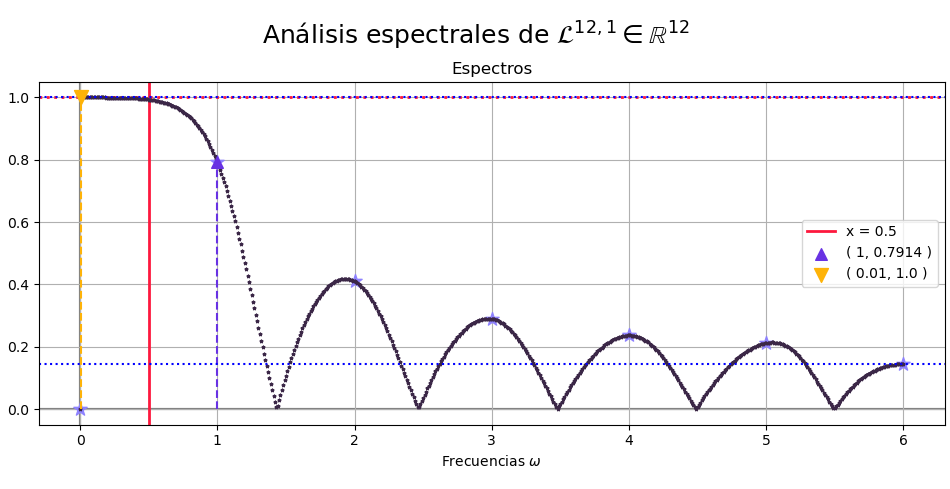
\includegraphics[scale = 0.5]{lim_1} 
\end{figure}	

\begin{figure}[H]
	\sidecaption{
	Observe que el espectro de $\cali{L}^{12,8}$ es, por el 
	contrario, continuo por $0$ pero discontinuo por $6$.
	\label{fig: lim 2}
	}
	\centering
	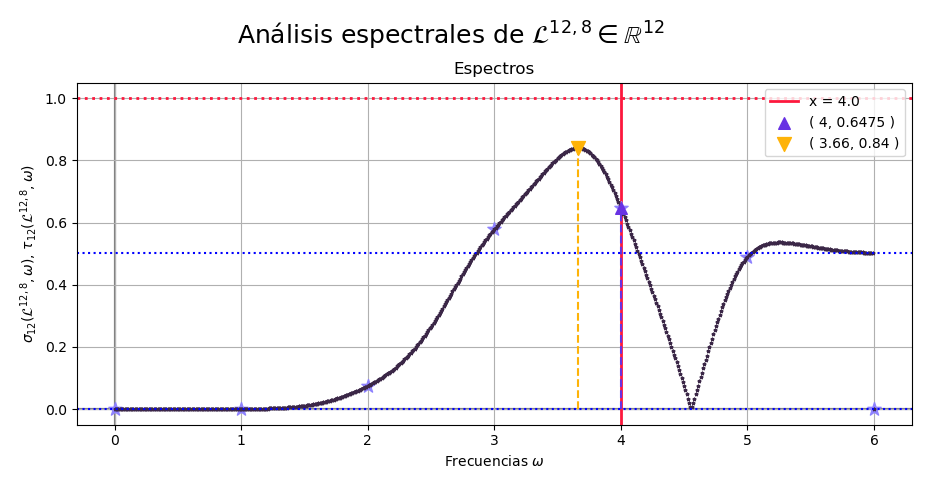
\includegraphics[scale = 0.5]{lim_2} 
\end{figure}

\begin{figure}[H]
	\sidecaption{
	El espectro de $\cali{L}^{12,9}$ es
	continuo por ambos extremos $0$ y $6$.
	\label{fig: lim 2}
	}
	\centering
	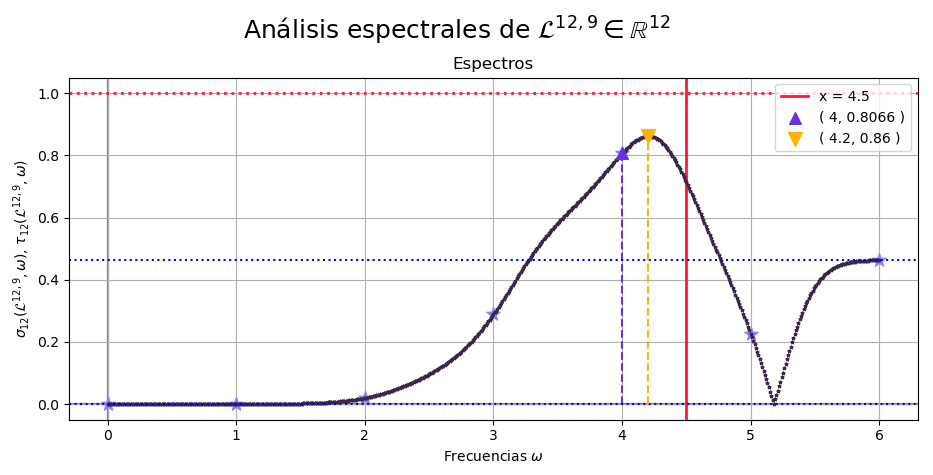
\includegraphics[scale = 0.5]{lim_3} 
\end{figure}

\begin{figure}[H]
	\sidecaption{
	El espectro de la señal
	$x = (1, 2, -3, -6) \in \IR^{4}$
	es discontinuo por ambos extremos
	$0$ y $2$.
	\label{fig: lim 4}
	}
	\centering
	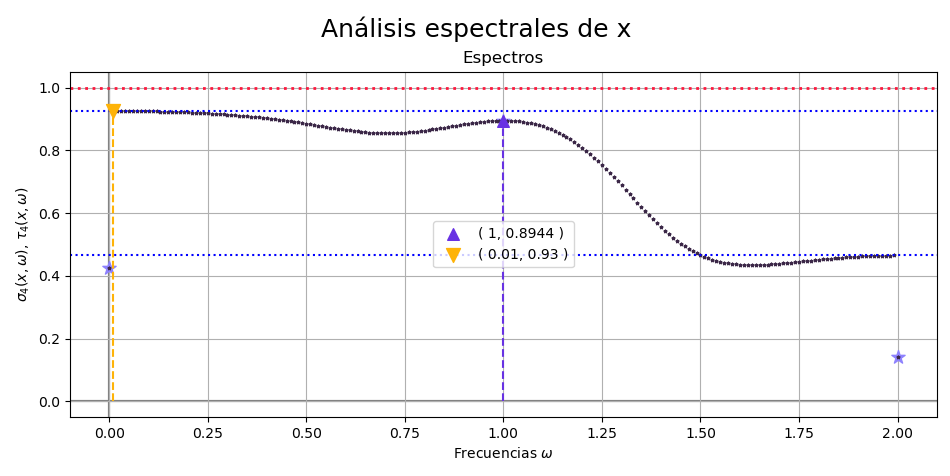
\includegraphics[scale = 0.5]{lim_4} 
\end{figure}


Vamos a terminar esta sección con expresiones
más sencillas (e ilustrativas) de los límites
laterales \eqref{eq: limite del espectro a cero}
y \eqref{eq: limite del espectro n medios}
de un espectro $\Sigma_{x}$.
Para ello necesitamos antes el siguiente
\begin{lema}
Sean $n \neq 2$, $x \in \IR^{n}$.
Si
\[
c_{i} := \langle x, \cali{L}^{m,i} \rangle,
\hspace{0.2cm} i = 0,1
\]
son los dos coeficientes primeros coeficientes
de $x$ respecto a la BLD $\cali{L}^{n,k}$,
entonces 
\begin{equation}
\label{ec: momento cero y coef 0}
M_{0}(x) = \sqrt{n} c_{0}
\end{equation}
y
 \begin{equation}
\label{ec: momento cero y coef 1}
M_{1}(x) = \frac{c_{1}}{\ell_{1}} + 
\frac{\sqrt{n}(n-1)}{2}c_{0},
\end{equation}
donde
\begin{equation}
\label{ec: l1}
\ell_{1}:= \sqrt{\frac{
12
}{(n-1)n(n+1)}}.
\end{equation}


Si 
\[
\tilde{c}_{i} := \langle x, (-1)^{m}\cali{L}^{m,i} \rangle,
\hspace{0.2cm} i = 0,1,
\]
entonces
\begin{equation}
\label{ec: momento cero y coef 0 tilde}
\tilde{M}_{0}(x) = \sqrt{n} c_{0}
\end{equation}
y
 \begin{equation}
\label{ec: momento cero y coef 1 tilde}
\tilde{M}_{1}(x) = \frac{c_{1}}{\ell_{1}} + 
\frac{\sqrt{n}(n-1)}{2}c_{0},
\end{equation}
\end{lema}
\noindent
\textbf{Demostración.}
En efecto, según la ecuación
\eqref{eq: Ln, 0, m}, 
\[
c_{0}= 
\langle x, \cali{L}^{m,0} \rangle
= \frac{1}{\sqrt{n}} \suma{m=0}{n-1}{x_{m}}
= \frac{1}{\sqrt{n}} M_{0}(x),
\]
luego, 
$M_{0}(x) = \sqrt{n} c_{0}$.
Además, según \eqref{eq: Ln, 1, m},
\[
c_{1}= 
\langle x, \cali{L}^{m,1} \rangle
= \ell_{1} \suma{m=0}{n-1}{x_{m} \left(
m-  \frac{n-1}{2}
\right)}
= \ell_{1} \left(
M_{1}(x)-\frac{n-1}{2}M_{0}(x)
\right);
\]
despejando a $M_{1}(x)$ y usando la relación dada
de $M_{0}(x)$ obtenemos 
\eqref{ec: momento cero y coef 1}.
Las demostraciones de 
\eqref{ec: momento cero y coef 0 tilde} y 
\eqref{ec: momento cero y coef 1 tilde} son
totalmente análogas.
\QEDB
\vspace{0.2cm}

En la siguiente proposición establecemos
una interesante relación entre el espectro de una señal $x$
con sus primeros dos coeficientes respecto a la base
de Legendre discreta $\cali{L}^{n}$.
\begin{prop}
\label{prop: relacion limite cero con legendre}
Sean $n \geq 2$, $x \in \IR^{n}$,
$\Sigma_{x}$ el espectro de $x$.
Si $W_{n,1}$ es como en \TODO{ref}, el espacio
de los polinomios discretos de grado $1$ y dimensión $n$, entonces
\begin{equation}
\label{eq: limite por cero como angulo}
\limite{\omega \rightarrow 0^{+}}{
\Sigma_{x}(\omega)} = \measuredangle(x, W_{n,1}).
\end{equation}
\end{prop}
\noindent
\textbf{Demostración.}
Según la proposición 
\ref{prop: proyecciones a espacios Wn,k}, 
\begin{equation}
\label{eq0: 25May23} 
||\Pi_{W_{n,1}}(x)|| = \sqrt{c_{0}^{2} + c_{1}^{2}}.
\end{equation}

Sustituyendo las expresiones 
\eqref{ec: momento cero y coef 0} y
\eqref{ec: momento cero y coef 1} en la expresión 
\eqref{eq: limite del espectro a cero} del límite para 
$\limite{\omega \rightarrow 0^{+}}{\Sigma_{x}(\omega)}$,
tenemos que
\begin{align*}
\limite{\omega \rightarrow 0^{+}}{\Sigma_{x}(\omega)^{2}}
= & 
\left(
\frac{
2M_{0}(x)^{2}(2n-1)(n-1) + 12M_{1}(x)^{2} - 12M_{0}(x)M_{1}(x)(n-1)
}{
||x||^{2} (n-1)(n+1)n}
\right)^{1/2} \\
= & \frac{1}{||x||^{2}
(n-1)(n+1)n
} 
\left(
2nc_{0}^{2}(n-1)(2n-1) + 12
\left(
\frac{c_{1}}{\ell_{1}} + 
\frac{\sqrt{n}(n-1)}{2}c_{0}
\right)^{2}-12
\sqrt{n} c_{0} \sqrt{\frac{12}{
(n-1)n(n+1)
}} 
\right) \\
= & \frac{1}{||x||^{2}
(n-1)(n+1)n}
\left(
(2n(n-1)(2n-1) + 3n(n-1)^{2}-6(n-1)^{2}n)c_{0}^{2}
+ \frac{12}{\ell^{2}_{1}}c_{1}^{2}
\right) \\
= & \frac{c_{0}^{2} + c_{1}^{2}}{||x||^{2}}.
\end{align*}

Usando \eqref{eq0: 25May23} podemos concluir
que
\[
\limite{\omega \rightarrow 0^{+}}{\Sigma_{x}(\omega)^{2}}
=  \frac{c_{0}^{2} + c_{1}^{2}}{||x||^{2}}
=  \frac{||\Pi_{W_{n,1}}(x)||}{||x||^{2}},
\]
siendo esta última expresión, según la proposición
\ref{prop: algunos hechos sobre el angulo entre un vector y un subespacio}, 
el coseno del ángulo que $x$ forma con $W_{n,1}$.  
\QEDB
\vspace{0.2cm}

Haciendo unos cambios de signo, se demuestra el resultado
análogo para el límite por la derecha de $n/2$ del espectro
$\Sigma_{x}$ de una señal $x \in \IR^{n}$.
\begin{prop}
\label{prop: relacion limite n medios con legendre}
Sean $n \geq 2$, $x \in \IR^{n}$,
$\Sigma_{x}$ el espectro de $x$.
Si $\tilde{W}_{n,1}$ es el espacio
\[
\tilde{W}_{n,1} := span \{ (-1^{m}\cali{L}^{n,0}_{m})_{m=0}^{n-1}, 
(-1^{m}\cali{L}^{n,1}_{m})_{m=0}^{n-1} \}
\]
entonces
\begin{equation}
\label{eq: limite por cero como angulo}
\limite{\omega \rightarrow \frac{n}{2}^{-}}{
\Sigma_{x}(\omega)} = \measuredangle(x, \tilde{W}_{n,1}).
\end{equation}
\end{prop}
\noindent
\textbf{Demostración.}
Sólo note que de la ortogonalidad de los
vectores $\cali{L}^{n,0}$ y $\cali{L}^{m,1}$
se sigue la de los vectores que por definición generan
al espacio $\tilde{W}_{n,1}$, 
luego, 
\begin{equation*}
||\Pi_{W_{n,1}}(x)|| = \sqrt{c_{0}^{2} + c_{1}^{2}}.
\end{equation*}
Haciendo cálculos análogos a los
de la demostración de la proposición 
\ref{prop: relacion limite cero con legendre} se llega
al resultado deseado.
\QEDB
\vspace{0.2cm}

\begin{comment}
Esta última proposición es importante, pues relaciona
el espectro de una señal 
con sus primeros dos coeficientes respecto a la base
de Legendre discreta $\cali{L}^{n}$. \\
Note que este es un resultado razonable, pues, por
definición del espectro $\Sigma_{x}$, si $\omega \geq 0$,
$\Sigma_{x}(\omega)$ es el coseno del ángulo que
$x$ forma con el espacio $P_{n, \omega} = 
span \left\{ cos \left(
2 \pi \omega\frac{m}{n}
\right)_{m=0}^{n-1},  
sen \left(
2 \pi \omega\frac{m}{n}
\right)_{m=0}^{n-1} \right\}$, y, conforme
$\omega$ tiende a cero por la derecha, 
las discretizaciones de coseno y seno que generan
el espacio $P_{n, \omega}$ tienden a ser las discretizaciones
de cosenos y senos de muy baja frecuencia, luego, intuitivamente
son las discretizaciones de las rectas tangentes de un coseno
y un seno en $t =0$, que son las rectas $y=1$
y $y =x$. Observe que discretizaciones de estas dos rectas
conforman una base para el espacio $W_{n,1}$.
\end{comment}
 
 
 
\section{Relación entre los espectros basados en la TDF y en espacios monofrecuenciales}

Después de todo lo expuesto en las secciones anteriores, tenemos
ya dos alternativas para realizar un análisis
espectral de una señal $x \in \IR^{n}$.

Sean $n \geq 2$, $M := \lceil \frac{n}{2} \rceil$, $x \in \IR^{n}$.
\begin{itemize}
	\item \textbf{(Espectro-0: basado en la TDF)} 
	Usando la transformada discreta de Fourier
	(c.f. sección \ref{sec: TDF}),
	el espectro de $x$ es la función
	\[
	\Tau_{x}: Dom_{TDF, n} \longrightarrow \IR^{+}_{0}
	\]	
	definida en \ref{def: espectro DFT}.
	
	La gráfica es entonces la de las frecuencias
	enteras $\omega$ dadas (dependiendo de la 
	paridad de $n$) por las
	tablas 6.1 y 6.2
	versus los coeficientes
	$\tau_{n}(x, \omega)$ definidos en
	\ref{def: taus}.
	
	Puesto que el realizar un análisis de 
	$x$ via la TDF significa encontrar una
	expresión de $x$ como una suma
	ponderada de muestreos de senos y cosenos,
	de frecuencias enteras las indicadas en las tablas 6.1 o 6.2,
	se tiene que  
	\begin{itemize}
		\item Para toda frecuencia $\omega$ considerada
		por la TDF,
		\[
		0 \leq \tau_{n}(x, \omega) \leq 1,
		\]
		y que
		\item entre más se acerque
		$\tau_{n, \omega}(x)$
		a $1$, mayor es la
		importancia de la frecuencia $\omega$ para
		sintetizar s $x$; recíprocamente, si 
		$\tau_{n}(x, \omega)$ es cercana a cero, entonces
		la frecuencia $\omega$ no es muy relevante para 
		sintetizar a la señal $x$.
	\end{itemize}
	\begin{defi}
	\label{def: FM0}
	Llamaremos \textbf{frecuencia principal-0}
	(y denotaremos por $FP0(x)$) 
	a una 
	frecuencia $\omega \in Dom_{TDF, n}$
	tal que, para cualquier otra $\omega' \in Dom_{TDF, n}$ 
	se tenga que 
	\[
	\tau_{n}(x, \omega') = \Tau_{x}(\omega^{'}) \leq
	\Tau_{x}(\omega) =  
	 \tau_{n}(x, \omega).
	\]
	\end{defi}
	Observe que tal frecuencia principal existe por ser 
	el máximo de un conjunto finito de números, pero que no 
	estamos asegurando que sea única. 
	
	\item \textbf{(Espectro-1: basado en espacios monofrecuenciales)} 
	Usando
	las ideas propuestas en 
	la sección
	\ref{sec: metodologia para realizar un analisis espectral que considere frecuencias arbitrarias}, 
	es decir, si se usan cosenos de ángulos a
	espacios monofrecuenciales $P_{n, \omega}$
	(c.f. \ref{eq: espacio Pnw}), el espectro
	de una señal $x$ se definió en
	\ref{def: espectro monofrecuenciales inicial}
	como la función 
	\[
	\Sigma_{x} : \left[0, \frac{n}{2} \right] \longrightarrow [0,1].
	\]
	
	La gráfica de este espectro es la de 
	las frecuencias $\omega \in [0, \frac{n}{2}]$ versus	
	los coeficientes
	$\sigma_{n}(x, \omega)$ definidos en 
	\ref{prp: ammm}. Observe que
	\begin{itemize}
		\item para cualquier frecuencia $\omega \geq 0$, se tiene que
		\[
		0 \leq \sigma_{n}(x, \omega) \leq 1
		\]
		\item 
	y, el que
	$\sigma_{n}(x, \omega)$ sea cercano a $1$ significa que un
	muestreo uniforme de un sinusoide de frecuencia $\omega$
	modela bien el comportamiento de $x$,
	mientras que un $\sigma_{n}(x, \omega)$ cercano
	a cero significa que 
	$x$ es casi perpendicular a toda señal de frecuencia $\omega$
	(c.f. nota \ref{nota: significado de los sigma en AE}).
	\end{itemize}
\end{itemize}

Nos gustaría, así como hicimos en la definición
\ref{def: FM0}, definir la frecuencia principal 
de una señal $x$ basada en el espectro
$\Sigma_{x}$ de esta. No es tan sencillo hacer esto, pues,
como comentamos en la sección
\ref{sec: simetria, periodicidad, continuidad}, 
tenemos expresiones para los límites del 
espectro $\Sigma_{x}$ de una señal $x$
en los puntos extremos $0$ y n/2,
pero estos límites no necesariamente coinciden con los
valores del espectro en tales puntos extremos,
por lo que intentar definir una
frecuencia principal como
\[
\omega \in [0, n/2] \textit{ tal que }
a_{x} = \Sigma_{x}(\omega), \textit{ donde }
a_{x} = sup \{ \Sigma_{x}(w): \hspace{0.2cm} \omega
\in [0, n/2] \}
\]
no es adecuado, pues no está excluida la 
posibilidad de que exista un espectro $\Sigma_{x}$
para el que no exista una $\omega \in [0, n/2]$ 
tal que $\Sigma_{x}(\omega) = a_{x}$, o sea, tal que 
$a_{x}$ que no sea máximo
del conjunto 
$\{ \Sigma_{x}(w): \hspace{0.2cm} \omega
\in [0, n/2] \}$. \\

\begin{figure}[H]
	\sidecaption{
	Se muestra un dibujo hipotético de un espectro
	$\Sigma_{x}$ para el que $a_{x} = 1$ pero no exista
	ninguna frecuencia $\omega \geq 0$ (una candidata
	a frecuencia principal) tal que $\Sigma_{x}(\omega) = a_{x}$.
 	\label{fig: ej FP1}
	}
	\centering
	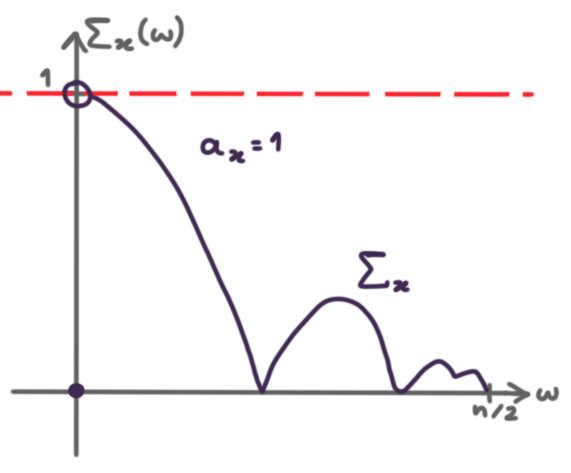
\includegraphics[scale = 1.4]{ejemplo_FP1.png} 
\end{figure}	
Sorteamos este problema si restringimos las frecuencias
$\omega$ a considerar a un subconjunto finito del
rango inicial de frecuencias
$[0, n/2]$.

\begin{defi}
	\label{def: FM1}
	Sean $n \geq 2$, $x \in \IR^{n}$. Sea
	$\cali{P}$ un subconjunto finito
	de $[0, n/2]$.
	Llamaremos la \textbf{frecuencia principal-$1$}
	(y denotaremos
	por $FP1(x)$) 
	de $x$ respecto al conjunto $\cali{P}$	
	a una frecuencia $\omega \in \cali{P}$ 
	tal que, para cualquier otra $\omega'$ del $\cali{P}$, se tenga que
	\[
	\sigma_{n, \omega'}(x) = \Sigma_{x}(\omega') 
	\leq \Sigma_{x}(\omega) = \sigma_{n, \omega}(x).
	\]
\end{defi}
En la práctica, el que se tenga que fijar un conjunto
finito $\cali{P} \subseteq [0, n/2]$ de frecuencias
para calcular la FP1 de una
señal $x$ no es un problema, pues ya teníamos que hacer
esto para calcular, de forma computacional, el espectro
$\Sigma_{x}$. Para respetar la convención
puesta en la nota 
\ref{nota: muestreo dom frecuencia}, vamos
a tomar a $\cali{P}$ como en 
\eqref{eq: malla frecuencias}.
	
\begin{nota}
Observe que no estamos asegurando
que las frecuencias principales
$FP0(x)$ y $FP1(x)$ como se definieron en 
\ref{def: FM0} y \ref{def: FM1}
sean únicas.
Si hay dos o más frecuencias $\omega'$ que satisfagan
la definición de frecuencia principal-0 
(resp. frecuencia principal-1), tomamos
como valor de $FP0(x)$ 
(resp. $FP1(x)$)
a la mayor de tales $\omega'$.
\end{nota}


Demostremos ahora que, de hecho, el espectro-0
de hecho es la restricción del espectro-1
al conjunto de frecuencias 
$Dom_{TDF, n}$ considerado por la transformada discreta
de Fourier.
\begin{prop}
\label{prop: coinciden espectr}
Sean $n \geq 2$, $x \in \IR^{n}$.
Sea $Dom_{TDF, n}$ el dominio del espectro-0 de $x$
como se definió en \ref{def. Dom tdf}. Se tiene que
\begin{equation}
\label{eq4: 4May}
\forall \omega \in Dom_{TDF, n}:
\hspace{0.2cm} \tau_{n}(x, \omega) = \sigma_{n}(x, \omega).
\end{equation}
\end{prop}

\noindent
\textbf{Demostración.}
Recuerde que los coeficientes
$\sigma_{n}(x, \omega)$
se definieron como
\[
\sigma_{n}(x, \omega) = \frac{|| \Pi_{P_{n, \omega}}(x) ||}{|| x ||}.
\]
Teniendo una base ortonormal del espacio 
$P_{n, \omega}$ puede calcularse la proyección involucrada en la fórmula
para $\sigma_{n}(x, \omega)$.
Recuerde que, por definición del espacio $P_{n, \omega}$,
\begin{itemize}
	\item los vectores $c_{n, \omega}$ y $s_{n, \omega}$ conforman
	una base de $P_{n, \omega}$ cuando $1 \leq \omega \leq M-1$ 
	(pues, para estos valores de omega se tiene siempre
	que $\omega \not\in \frac{n}{2} \IZ$) y
	\item $c_{n, \omega}$ conforma una base 
	de $P_{n, \omega}$ cuando $\omega = 0$ y,
	en el caso en el que $n$ es par, también para cuando $\omega = M$
	(pues sólo para estos valores de omega se tiene 
	que $\omega \in \frac{n}{2} \IZ$).
\end{itemize}
Además, según la proposición
\ref{prop: base de fourier version real},
para todas estas $\omega$,
los vectores de la lista anterior son ortogonales entre
sí y tienen norma uno, luego, más que una base de 
$P_{n, \omega}$ constituyen una BON para este espacio.
Así, $\Pi_{P_{n, \omega}}(x)$ puede encontrarse 
simplemente calculando los productos punto 
de $x$ con los elementos de estas BONs (c.f. 
nota \ref{nota: sobre la identidad de parseval});
comparando este cálculo con la definición 
\ref{def: taus}
de los coeficientes $\tau_{n}(x, \omega)$,
concluimos que en efecto se
tiene la iguadad \eqref{eq4: 4May}.

\QEDB
\vspace{0.2cm}

Así, \textbf{el espectro basado en espacios monofrecuenciales
es una extensión de la definición del espectro 
basado en la transformada discreta de Fourier}.
Como ya recordamos al inicio, la
ventaja de este primer espectro es que para calcularlo es posible usar
un rango cualquiera de frecuencias no negativas, mientras que el segundo, 
a pesar de que da no sólo un proceso de análisis de una señal 
de $x$ a partir de sinusoides, sino también uno de síntesis
(c.f. nota \ref{nota: ya?}), se limita a considerar las frecuencias 
en $Dom_{TDF, n}$. \\

Recuerde que en la nota 
\ref{nota: muestreo dom frecuencia} explicamos que 
basta evaluar a $\Sigma_{x}$ en el intervalo $[0, n/2]$, 
pues a partir de estos valores puede deducirse el valor
del espectro en cualquier otra frecuencia positiva; observe que,
para toda $n$, el conjunto de frecuencias enteras 
consideradas por la TDF, $Dom_{TDF, n}$, está
contenido en $[0, n/2]$, luego, basta calcular 
a $\Sigma_{x}$ en $[0, n/2]$
para tener ambos análisis espectrales.


\begin{nota}
\label{nota: la mejor frecuencia}
Fijados $n \geq 2$
y $x \in \IR^{n}$, \textbf{entre más cercano a $1$ sea 
el coeficiente 
$\sigma_{n}(x, \omega)$, mejor es usar un sinusoide
de frecuencia $\omega$ para ajustar la gráfica de $x$}.
Esto porque, recuerde, entre más cercano a uno sea uno de
esos coeficientes, más cercana estará la señal $x$ 
al espacio monofrecuencial $P_{n, \omega}$, luego, más
cercana está $x$
a tener
la propiedad de ser una discretización de un sinusoide
de la respectiva frecuencia $\omega$.
\end{nota}

\begin{nota}
\label{nota: proyeciones monof TDF}
Sea $x \in \IR^{n}$; sea 
\eqref{ec: sintesis 0} o 
\eqref{ec: sintesis 1}
(dependiendo de la paridad de $n$)
la síntesis de $x$ respecto a la base de Fourier
real $\cali{F}_{n}$. De esta suma, podemos
separar los sumandos que corresponden a una
cierta frecuencia $\omega \in Dom_{TDF, n}$; recordando
que, como se notó
en la demostración de la proposición
\ref{prop: coinciden espectr}, 
los correspondientes vectores
de frecuencia $\omega$ (que son ya sea uno o dos, dependiendo del valor
de $\omega$) conforman una BON para el correspondiente
espacio monofrecuencial 
$P_{n, \omega}$, tenemos que la parte de la 
síntesis de $x$ que corresponde a 
cierta frecuencia $\omega$ es igual a
$\Pi_{P_{n, \omega}}(x)$. \\

Aplicando esto al ejemplo \ref{ej: DFT1},
si $x$ es la señal definida en 
\ref{eq2: 10ab}, se tiene que
\[
\Pi_{7, 0} = 4.12 c_{7,0}, 
\]
\[
\Pi_{7, 1} = -8.76 c_{7,1} - 7.35 s_{7,1}, 
\]
\[
\Pi_{7, 2} = 4.77 c_{7,2} - 10 s_{7,2}, 
\]
\[
\Pi_{7, 3} = 0.14 c_{7,3} + 9.91 s_{7,z3}.
\]
\end{nota}



\begin{ejemplo}
\label{ej: espectros comparacion}

Sea $f_{\omega}$
el sinusoide definido como
\begin{equation}
\label{eq: sinusoide eje}
f_{\omega}(t) := -1.5 cos (2 \pi \cdot \omega t + 2 \pi \cdot 0.2).
\end{equation}
Considere a una señal $x \in \IR^{16}$ que sea el resultado
de muestrear uniformemente al sinusoide
$f_{3.4}$
con ruido aleatorio 
(con distribución, pongamos, uniforme en $[-0.5, 0.5]$).

A continuación, mostramos las gráficas
de los espectros de $x$. Para
calcular el espectro $\Sigma_{x}$,
usamos el dominio
establecido en la nota 
\ref{nota: muestreo dom frecuencia}.

\begin{figure}[H]
\centering
	\sidecaption{ De ahora en adelante, siempre que
	grafiquemos espectros,usaremos los colores y notaciones
	de esta figura. \label{fig: ejemplo_comparacion}}
    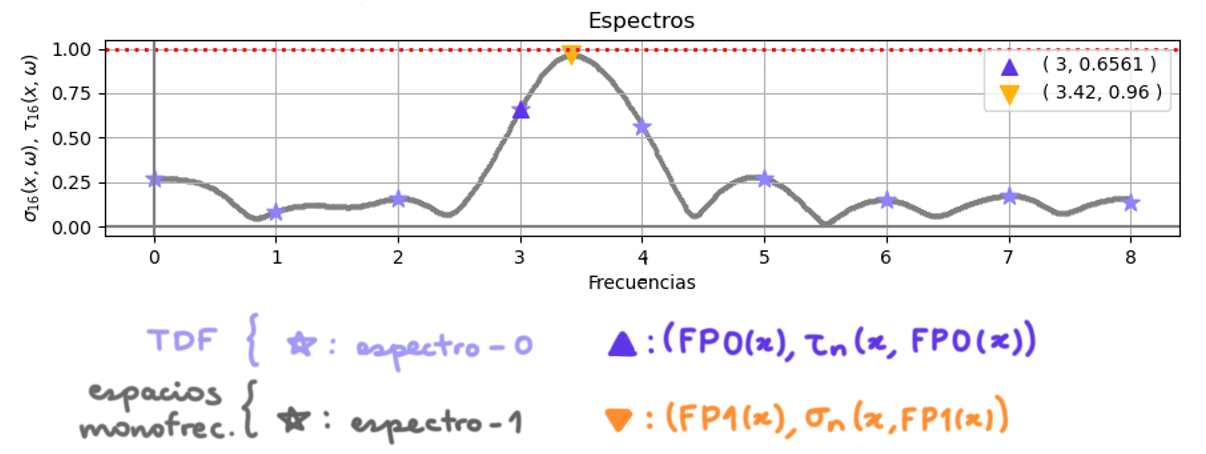
\includegraphics[scale = 1]{./estudios_espectrales/ejemplo_comparacion_1}
\end{figure}


Observe cómo el espectro-$1$ parece completar la información
dada por el espectro-$0$, pues, a diferencia del primero,
el espectro-$0$
da coeficientes de frecuencia $\tau_{n}(x, \omega)$ sólo
para algunas frecuencias enteras $\omega$, mientras que en el espectro-$1$
es posible considerar cualesquiera frecuencias $\omega \geq 0$; como puede observar
en la gráfica, 
\[
FP0 (x) = 3 \hspace{0.2cm} \textit{y} \hspace{0.2cm}
FP1 (x) = 3.42;
\]
esta segunda frecuencia es mucho más cercana a
la frecuencia $\omega =3.4$ del sinusoide del que
fue obtenida la señal $x$; como agregamos ruido
aleatorio en las mediciones, no 
es de extrañarse que no se haya
obtenido exactamente $FP1(x) = 3.4$.

A pesar de que el espectro-$0$, el obtenido a partir de la
transformada discreta de Fourier, no dio una mala estimación (del rango
de frecuencias $Dom_{TDF,n}$ considerado por esta herramienta,
$\omega =3$ es el valor más cercano al valor real $\omega = 3.4$), vemos en este
ejemplo que usando el espectro-$1$ es posible obtener mejores
estimaciones de frecuencias que modelen a la señal original. \\

Mostramos ahora la gráfica de $x$ junto con
\begin{itemize}
	\item la parte de la síntesis de $x$ respecto a la $TDF$
	que corresponde a la frecuencia principal
	$FP0(x)$ (c.f.
	nota \ref{nota: ya?}), que de hecho,
	según la nota \ref{nota: proyeciones monof TDF}, es
	$\Pi_{P_{36,3}}(x)$
	\begin{figure}[H]
			\sidecaption{
			Puesto que $\{ c_{36, 3}, s_{36, \omega} \}$
			es una BON de $P_{36, 3}$, claro que la señal 
			que resulta de discretizar el sinusoide morado en la malla
			$I_{36}$ es, de hecho, la proyección de $x$ 
			al espacio monofrecuencial $P_{36, 3}$.
 			\label{fig: comparacion 2}
			}
			\centering
			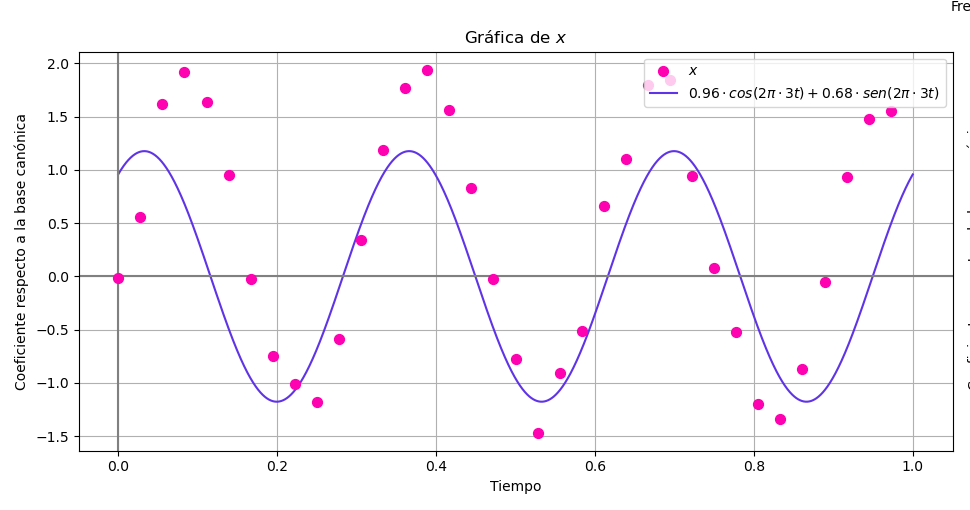
\includegraphics[scale = 0.5]{./estudios_espectrales/ejemplo_comparacion_2} 
		\end{figure}		
	
	y
	\item la señal $\Pi_{P_{16, 3.42}}(x)$, o sea, la señal de
	dimensión $16$ y frecuencia $FP1(x)=3.42$ más cercana a $x$, junto con
	el sinusoide continuo del que fue muestreado.
	\begin{figure}[H]
			\sidecaption{
			Para obtener la versión continua del sinusoide 
			discreto $\Pi_{P_{36, 3.42}}(x)$ (i.e. la gráfica naranja),
			usamos las fórmulas establecidas en los teoremas
			\ref{teo: amelie1} y \ref{teo: amelie2}.
			\label{fig: comparacion 3}
			}
			\centering
			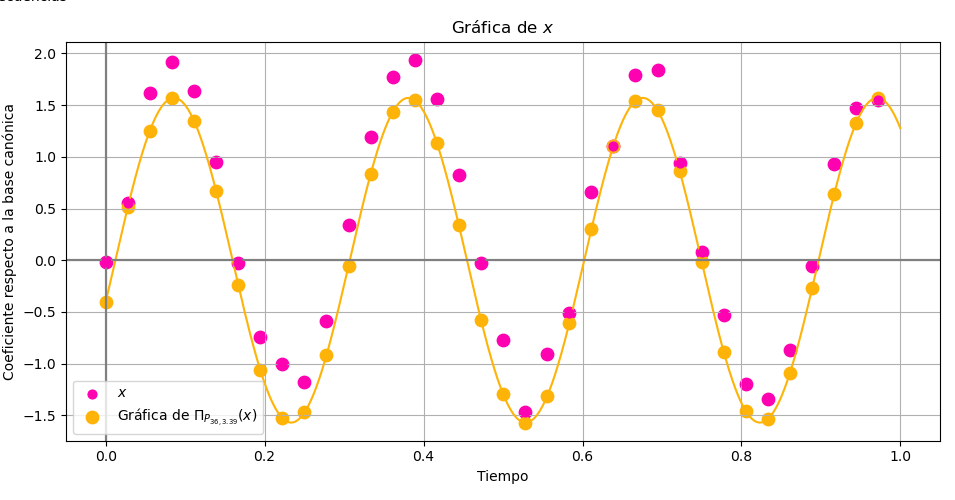
\includegraphics[scale = 0.5]{./estudios_espectrales/ejemplo_comparacion_3} 
		\end{figure}		
\end{itemize}


Los sinusoides de las figuras \ref{fig: comparacion 2} y
\ref{fig: comparacion 3}
son las señales de frecuencia pura
$3$ y $3.42$, respectivamente, cuya distancia euclidea
a la señal original $x$ es mínima. Observe que la segunda
señal, aquella cuya frecuencia
fue determinada
a partir del estudio espectral basado en espacios
monofrecuenciales,
parece ajustarse un poco mejor a la gráfica de $x$. \\

\begin{figure}[H]
			\sidecaption{
			Mostramos ahora los espectros de la señal $x$ que se obtiene
			tomando $36$ muestras uniformemente espaciadas del mismo sinusoide
			$f_{3.4}(t)$, 	
			esta vez sin agregar ruido aleatorio a las mediciones.
			Observe que el espectro-1 detectó a la frecuencia $\omega = 3.4$
			como la mejor, y que el sinusoide naranja ajusta perfectamente la gráfica
			de $x$. Como la frecuencia real no es entera, usar la frecuencia principal
			dada por la TDF sigue sin dar resultados perfectos, aunque no malos.
			\label{fig: sinusoide sin ruido}
			}
			\centering
			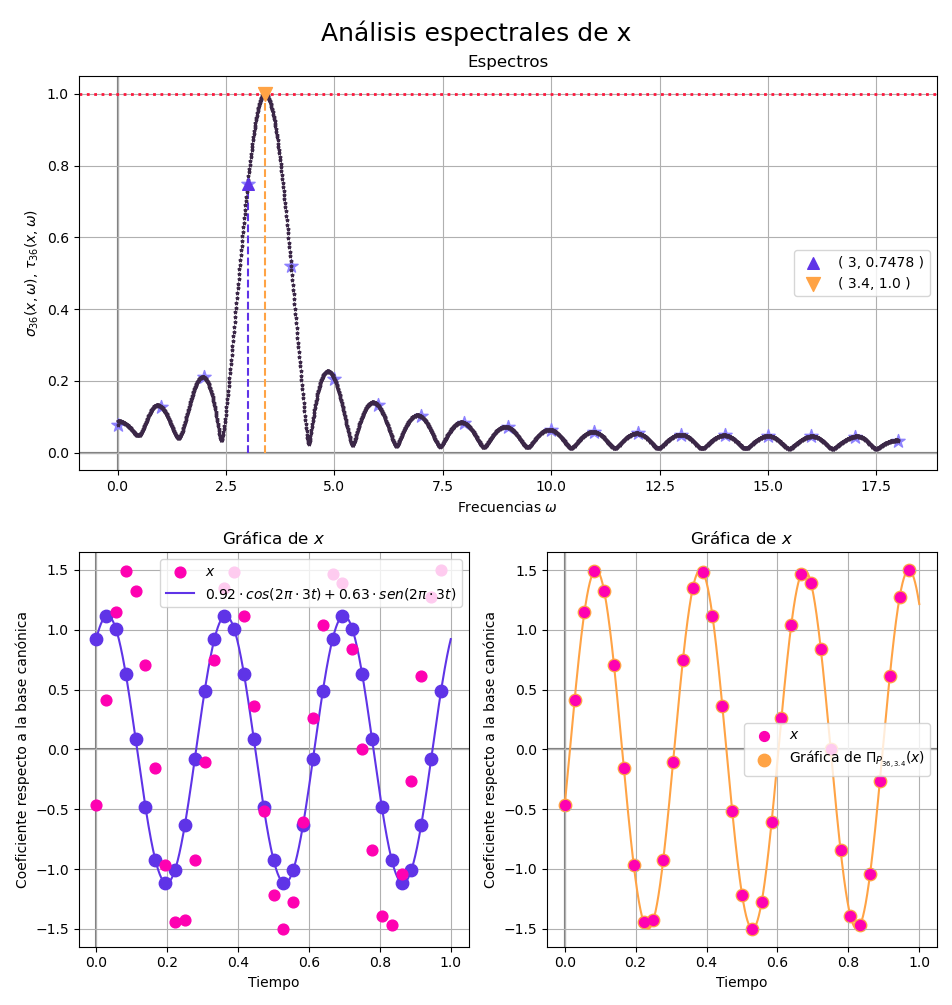
\includegraphics[scale = 0.4]{./estudios_espectrales/sinusoide_sin_ruido} 
		\end{figure}		



	\begin{figure}[H]
			\sidecaption{
			Si ahora muestreamos sin ruido
			del sinusoide $f_{5}$,
			como 
			era de esperarse, la frecuencia principal de ambos
			espectros es $5$
			(y el valor de los 
			espectros en tal frecuencia
			es igual a $1$, la cota
			superior). Además, 
			las gráficas de frecuencia $5$ que resultan
			ajustan a la perfección a la señal original $x$.
			\label{fig: comparacion 4}
			}
			\centering
			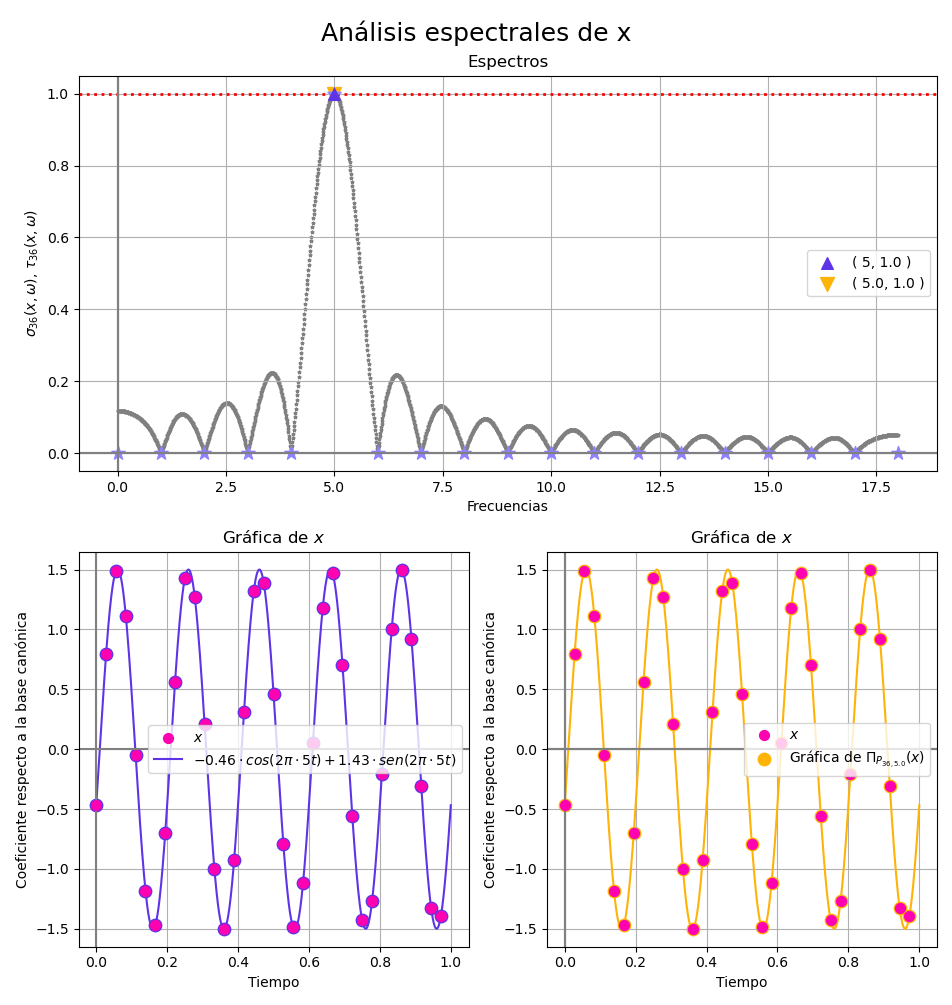
\includegraphics[scale = 0.4]{./estudios_espectrales/ejemplo_comparacion_4} 
		\end{figure}	


Para terminar este ejemplo, tomemos una suma de sinusoides
de varias frecuencias, digamos, de frecuencias
$1$, $4$ y $7$; sea
\[
g(t) = 3 sen(2 \pi t) + sen(2 \pi \cdot 4t) + 0.5 cos(2 \pi \cdot 7t).
\]
Sea $x$ la señal que resulta de muestrar, sin ruido, este sinusoide
$g$, siendo $25$ el tamaño de la muestra.
\begin{figure}[H]
	\sidecaption{
	En la imagen se muestran los espectros de tal $x$. Observe que los
	espectros parecen concentrarse alrededor de las 
	frecuencias $1$, $4$ y $7$.
	\label{fig: sin varias frec}
	}
	\centering
	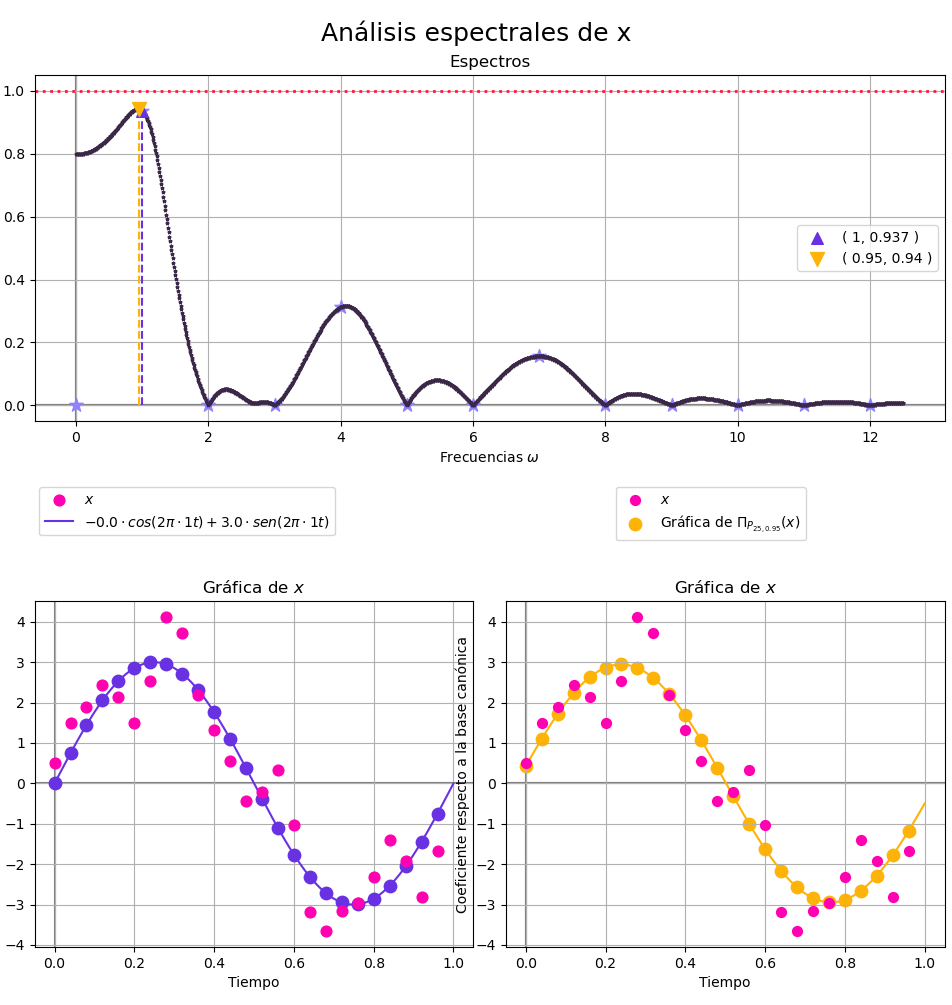
\includegraphics[scale = 0.4]{./estudios_espectrales/sinusoide_varias_frecuencias} 
\end{figure}	

\final
\end{ejemplo}

\subsection{Adaptación del análisis espectral a señales reales con una frecuencia de muestreo dada}

Para hacer nuestros análisis espectrales, hemos
usado la dimensión $n$ del PDL $\cali{L}^{n, k} \in \IR^{n}$
en cuestión
para buscar, en base a máximos globales
del espectro 
$\Sigma_{x}: [0, \frac{n}{2}] \longrightarrow [0,1]$, la
mejor frecuencia $\omega$ para aproximar la gráfica
de $\cali{L}^{n,k}$ en base a un sinusoide discreto
de dimensión $n$. \\


Note que en esa discusión nunca hablamos de 
parámetros importantes para, de forma canónica, hacer
un análisis espectral, como lo son la
duración en tiempo de la señal o la frecuencia
de muestreo.

\begin{defi}
\label{def: tiempo y frec de muestreo}
La cantidad de muestras tomadas (de forma uniforme)
de una señal por unidad de tiempo 
será denotada por $F_{s}$ y llamada \textbf{frecuencia
de muestreo} de la señal. A la cantidad de unidades de
tiempo que dura la medición se le denotará por $T$. \\

A la cantidad total de muestras tomadas se le denotará
por $L$.
\end{defi}
Observe que, para poder dividir una unidad
de tiempo en $F_{s}$ subintervalos de igual longitud,
se deben divider al eje del tiempo con los puntos
\begin{equation}
t_{k} := t_{0} + h k, \hspace{0.2cm}
\textit{con } h := \frac{1}{F_{s}}.
\end{equation}
A tal constante $h$, definida como el recíproco de la frecuencia
de muestreo, se le llama el \textbf{paso temporal} de la señal. \\

De las definiciones se sigue de inmediato que
\begin{equation}
\label{eq: relacion L, T Fs}
L = T F_{s}.
\end{equation}
\begin{figure}[H]
	\sidecaption{
	Adoptamos la convención de empezar a medir 
	un bloque de $F_{s}$ mediciones desde que inicia la
	unidad de tiempo (que, en el caso de la figura, se ha
	fijado como segundos).
	\label{fig: Fs 1}
	}
	\centering
	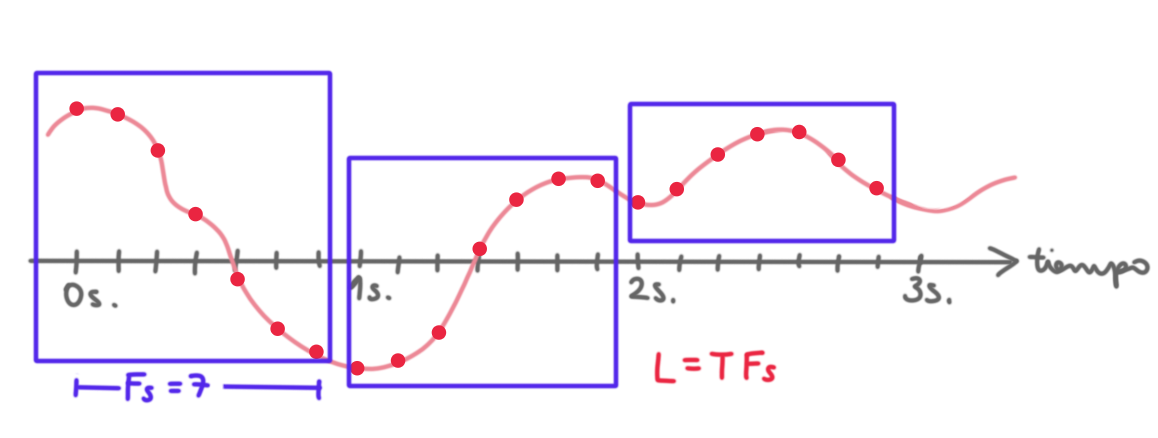
\includegraphics[scale = 1]{Fs_1} 
\end{figure}	

Nosotros, por el momento, sólo nos
hemos enfocado en buscar
una frecuencia $\omega \in [0, \frac{n}{2}]$ que de lugar
a un sinusoide que aproxime bien la gráfica
de $\cali{L}^{n,k}$;
observe que, al hacer esto, hemos supuesto de forma
implícita que estamos estudiando una señal
de duración una unidad de tiempo
($T = 1$) de longitud $n$
(o sea, $L = F_{s} = n$). \\
Supongamos ahora que
tenemos una señal $x$ que consta de $L$ mediciones, siendo
$F_{s}$ la frecuencia de muestreo.
\begin{figure}[H]
	\sidecaption{
	Para la imagen, hemos fijado $F_{s}= 10$
	y $L = 40$.
	\label{fig: frecuencia 1}
	}
	\centering
	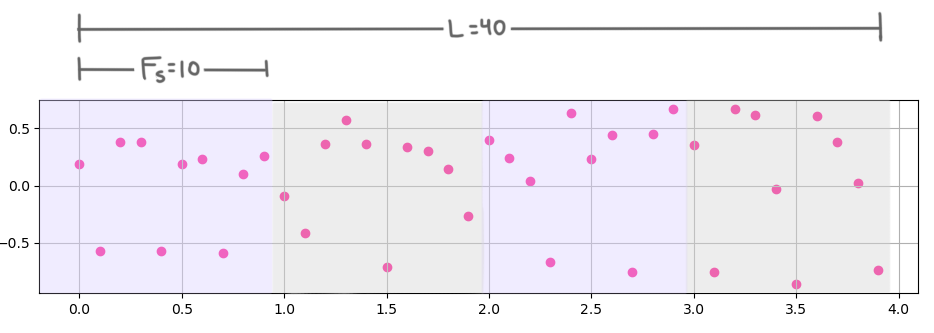
\includegraphics[scale = 0.45]{frecuencia_1} 
\end{figure}	

Sea ahora $2 \leq n \leq L$ y
supogamos que
se hizo el análisis
espectral 
de una sección $x_{|n}$ de tal señal
que conste de $n$ puntos
(usando el espectro
$\Sigma_{x}: [0, \frac{n}{2}]
\longrightarrow [0,1]$).
Digamos que, como conclusión de ese análisis, se
obtuvo que un sinusoide de frecuencia $\omega \in [0, \frac{n}{2}]$
ajusta bien \textit{esa sección particular 
$x_{|n}$
de la señal $x$}.
\begin{figure}[H]
	\sidecaption{
	Para la imagen, hemos fijado $n= 6$;
	se calculó que la mejor frecuencia para ajustar 
	los primeros $6$ puntos que componen la señal
	original $x$ es $w = 2$.
	\label{fig: frecuencia 2}
	}
	\centering
	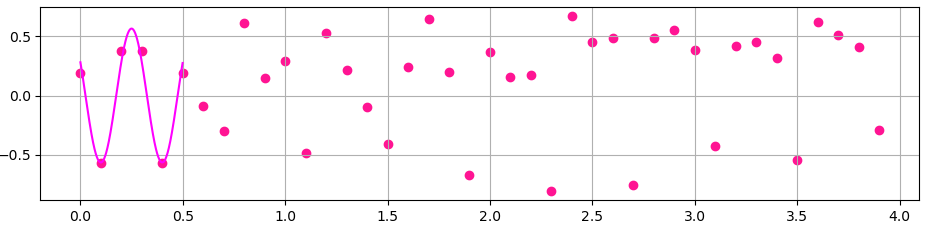
\includegraphics[scale = 0.45]{frecuencia_2} 
\end{figure}	

Observe que, en general, si se quisiera usar
directamente una frecuencia de $w$ para ajustar
a la señal $x$, la aproximación lograda en los
$n$ puntos escogidos previamente puede no ser válida.
\begin{figure}[H]
	\sidecaption{
	Usando los datos de la figura \ref{fig: frecuencia 2}, podriamos
	intentar en un principio usar a un sinusoide de frecuencia $2$
	para intentar modelar a la señal, pero un sinusoide de tal frecuencia,
	como es el caso de esta figura, puede que ni siquiera sea adecuado
	para modelar el pedazo $x_{|n}$ original a partir del cual se obtuvo
	la frecuencia $\omega$.
	\label{fig: frecuencia 2}
	}
	\centering
	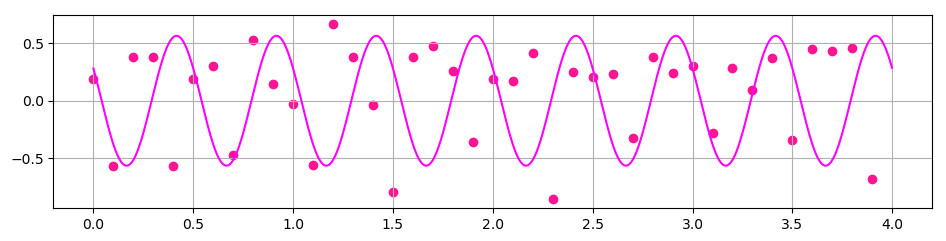
\includegraphics[scale = 0.45]{frecuencia_3} 
\end{figure}
Esto se debe a que	
tal frecuencia $\omega$ es buena para aproximar
a dichos $n$ puntos cuando se ha tomado como
unidad de tiempo a $n$, pero, 
por la forma en que fue muestreada la señal original $x$,
son $F_{s}$ (y no necesariamente $n$) la cantidad de puntos
que conforman una unidad. Así, puesto que con $\omega$
ciclos de un sinusoide se aproximaron $n$ puntos, 
la frecuencia que debe escogerse para aproximar a todos los $L$
puntos es
\begin{equation}
\label{eq: rel frecuencia real y ficticia}
\tilde{w} := \frac{F_{s}}{n} \omega.
\end{equation}

\begin{figure}[H]
	\sidecaption{
	Es con una simple regla de tres que se deduce
	la relación \eqref{eq: rel frecuencia real y ficticia}.
	\label{fig: frecuencia real}
	}
	\centering
	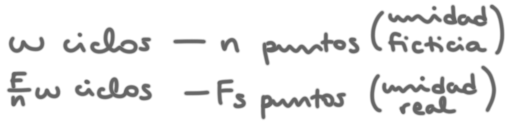
\includegraphics[scale = 1.4]{frecuencia_real} 
\end{figure}	
\begin{figure}[H]
	\sidecaption{
	Según los datos de las figuras
	\ref{fig: frecuencia 1}
	y \ref{fig: frecuencia 2}, con un sinusoide de frecuencia
	$\tilde{\omega} = 10/3$ se aproximan bien a los seis
	puntos en base a los cuales se encontró a la primera
	frecuencia $\omega$.
	\label{fig: frecuencia 4}
	}
	\centering
	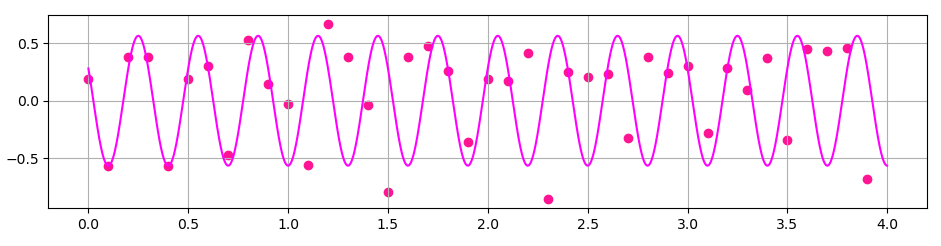
\includegraphics[scale = 0.45]{frecuencia_4} 
\end{figure}